%%-----------------------------------------------------------------------------------------------------------------------
% AGU Template
\documentclass[draft]{agujournal2019}
\usepackage{url} %this package should fix any errors with URLs in refs.
\usepackage{lineno}
%\usepackage[inline]{trackchanges} %for better track changes. finalnew option will compile document with changes incorporated.
\usepackage{soul}
\linenumbers
%%%%%%%
% As of 2018 we recommend use of the TrackChanges package to mark revisions.
% The trackchanges package adds five new LaTeX commands:
%
%  \note[editor]{The note}
%  \annote[editor]{Text to annotate}{The note}
%  \add[editor]{Text to add}
%  \remove[editor]{Text to remove}
%  \change[editor]{Text to remove}{Text to add}
%
% complete documentation is here: http://trackchanges.sourceforge.net/
%%%%%%%

%\draftfalse

\journalname{Journal of Advances in Modeling Earth Systems (JAMES)}

%\usepackage{natbib}
\usepackage{graphicx}
\usepackage{booktabs}
\usepackage{amsmath,amssymb,amsfonts,amscd,amsthm}
\usepackage{bm}
\usepackage{pdflscape}
\usepackage[flushleft]{threeparttable}
\usepackage{lineno}
\usepackage{setspace}
\usepackage{textcomp}
\usepackage{times}
\usepackage{enumerate}
\usepackage{rotating}

%%%%% units %%%%%
\usepackage{siunitx}
\sisetup{output-exponent-marker=\ensuremath{\mathrm{e}}}
\DeclareSIUnit\yr{yr}

%%%%% personal definitions %%%%
% vectors and matrices
\renewcommand{\vec}[1]{\mathbf{#1}}
\newcommand{\tens}[1]{\mathrm{#1}}
\newcommand{\id}{\tens{Id}}

% integrals
\newcommand{\deriv}[1]{\frac{\mathrm{d}}{\mathrm{d}#1}}
\newcommand{\dd}[1]{\,\mathrm{d}#1}

% limits and sums
\newcommand{\intl}{\int\limits}
\newcommand{\suml}{\sum\limits}

% spaces
\newcommand{\R}{\mathbb{R}}


\begin{document}
%
%\noindent
%{\bf Keywords}: carbon cycle models, carbon stocks, carbon fluxes, reservoir theory, compartment models, radiocarbon, dynamical systems,  model diagnostics
%

\title{Mathematical reconstruction of land carbon models from their numerical output: computing soil radiocarbon from $^{12}$C dynamics}

\authors{Holger Metzler\affil{1},
              Qing Zhu\affil{2}, 
              William Riley\affil{2}, 
              Alison Hoyt\affil{1,2}, 
              Markus M\"uller\affil{1}, 
              Carlos A. Sierra\affil{1}}

\affiliation{1}{Max Planck Institute for Biogeochemistry, Hans-Kn\"oll-Str. 10, 07745 Jena, Germany}
\affiliation{2}{Climate and Ecosystem Sciences Division, Lawrence Berkeley National Laboratory, Berkeley 94720, USA}

\correspondingauthor{C.A. Sierra}{csierra@bgc-jena.mpg.de}

%\begin{keypoints}
%\item enter point 1 here
%\item enter point 2 here
%\item enter point 3 here
%\end{keypoints}

\begin{abstract}
Radiocarbon (\textsuperscript{14}C) is a powerful tracer of the global carbon cycle that is commonly used to assess carbon cycling rates in various Earth system reservoirs and as a benchmark to assess model performance. Therefore, it has been recommended that Earth System Models (ESMs) participating in the Coupled Model Intercomparison Project Phase 6 (CMIP6) report predicted radiocarbon values for relevant carbon pools. However, a detailed representation of radiocarbon dynamics may be an impractical burden on model developers. Here, we present an alternative approach 
to compute radiocarbon values from the numerical output of an ESM that does not explicitly represent these dynamics. The approach requires computed \textsuperscript{12}C stocks and fluxes among all carbon pools for a particular simulation of the model. From this output, a time-dependent linear compartmental system is computed with its respective state-transition matrix. Using transient atmospheric \textsuperscript{14}C values as inputs, the state-transition matrix is then applied to compute radiocarbon values for each pool, the average value for the entire system, and component fluxes. We demonstrate the approach with ELMv1-ECA, the land component of an ESM model that explicitly represents \textsuperscript{12}C and \textsuperscript{14}C in seven soil pools and ten vertical layers. Results from our proposed method are highly accurate (relative error $<$ 0.01\%) compared with the ELMv1-ECA \textsuperscript{12}C and \textsuperscript{14}C predictions, demonstrating the potential to use this approach in CMIP6 and other model simulations that do not explicitly represent \textsuperscript{14}C. 
%Furthermore, since the method provides a linear reconstruction of the model for a particular simulation, it can also be used to calculate other system-level metrics such as ages and transit times, carbon storage capacity and potential, and perform traceability analyses.
\end{abstract}

\section*{Plain Language Summary}
%[ enter your Plain Language Summary here or delete this section]
Models representing ecosystem carbon dynamics are generally complex and difficult to analyze. Comparing
different models with different structures is even more challenging due to the variety of processes represented
in the models. However, it is possible to use the numerical output of models to reconstruct the original structure
using a common mathematical framework. In this manuscript, we demonstrate this approach and apply it to compute
radiocarbon dynamics of a land carbon model. The proposed approach can reconstruct the carbon and radiocarbon
dynamics of the original model very accurately, and can be used to study system-level dynamics of complex contrasting models.


\section{Introduction}
Terrestrial ecosystems, and soils in particular, are important global carbon (C) reservoirs but with large uncertainties in the size of the stock, process rates, and their representation in Earth System Models (ESMs) \cite{Luo2016,Sulman2018B}. The dynamics of radiocarbon in various components of terrestrial ecosystems can be used to interpret the rates at which CO$_2$ is removed from the atmosphere into plants through photosynthesis, moves from vegetation into soils through litter fall and mortality, and finally cycles back to the atmosphere via respiration. As a result, radiocarbon has been used in many empirical studies to evaluate rates of soil C cycling, and more recently, as a tool for model evaluation \cite{Chen2009JGR,Dwivedi2018SBB,Ahrens2015SBB} and inter-comparison \cite{He2016}. 

Measurements of radiocarbon offer great potential to constrain temporal dynamics of the land carbon cycle in ESMs as well as to assess their performance. However, to date, such comparisons have been limited to a small number of models that simulate C isotopes \cite<e.g.>{Koven2013, Tifafi2018,Chen2009JGR}, as the majority of models do not explicitly represent isotope dynamics. The current coupled climate-carbon cycle model inter-comparison project (C4MIP) of the Coupled Model Inter-comparison Project Phase 6 (CMIP6) requests model participants to explicitly model radiocarbon and include the corresponding output from the major land and ocean model compartments \cite{Jones2016, Graven2017}. However, this additional request can be time-consuming to implement, and computationally intensive to run. Thus, the goal of this work is to develop a tool to make radiocarbon-based comparisons of C cycling practical and comparable across different ESMs even if they do not explicitly include these dynamics.

The availability of radiocarbon output from a range of models would allow an additional comparison and evaluation against global datasets, such as the International Soil Radiocarbon Database (ISRaD) \cite{Lawrence2019}, and would provide a new way to differentiate patterns of C cycling across different model structures \cite{Sierra2014}. There are literally hundreds of models of soil carbon cycling described in the literature \cite{Manzoni2009SBB}, each relying on different hypotheses about internal system dynamics, with specific model structures and parameterizations. Generalizations of models have also been proposed based on basic assumptions of soil organic matter dynamics \cite{Sierra2015}. Computing radiocarbon output from these different classes of models, without the need to incorporate explicit isotopes dynamics in the model, would benefit data-model comparisons, and improve the understanding of soil C dynamics in these models.

Linear response theory suggests that the impulse response function of a particular model can be used to compute isotope dynamics without explicitly simulating the isotope within the model, but rather using the response function to convolve the isotope tracers \cite{Thompson1999}. Therefore, it may not be necessary to explicitly represent isotope dynamics a priori in a model; rather, they can be obtained a posteriori through the convolution procedure. However, linear response theory relies on assumptions of steady-state and model linearity, which are not met for the type of transient simulations performed with ESMs. 

\citeA{Metzler2018PNAS} recently developed a method to obtain a mathematical object, the state-transition matrix (see details below), which generalizes response function theory for nonlinear models out of equilibrium. This approach removes previous assumptions that prevented the use of the linear response approach for the computation of isotope and tracer dynamics a posteriori from simulations. Therefore, the state-transition matrix approach offers an opportunity to compute isotope dynamics from models that do not explicitly represent them, and could be applied to models participating in CMIP6, for example. However, since output from these models is provided in discrete time steps often much larger than the internal model time step, it is a challenge to translate the state-transition-matrix approach from the continuous to the discrete case.

We introduce in this manuscript an approach to mathematically reconstruct land carbon models from simulation output, and use the reconstruction to compute radiocarbon values. To this end, we extend the method presented in \citeA{Metzler2018PNAS} for the reconstruction of a differential equation model from an existing solution and the computation of the state-transition matrix in continuous time. We show how to translate the approach to the discrete-time case, and apply it to reconstruct tracer and isotope dynamics from model output. We first give a mathematical overview of the approach and then present examples of its use. We test our approach by comparing our computed values to output from the ELMv1-ECA model \cite{Zhu2019, Riley2018,Chen2009JGR, Tang2018EI}, the land component of the Exascale Earth System Model (E3SM) model, which explicitly represents radiocarbon and is therefore an appropriate test case to evaluate our proposed method. We evaluate the modeled radiocarbon values along the entire vertically resolved soil profile, and across all represented soil and litter pools over time. We believe this new framework has  potential for application to the CMIP6 simulations and to models with more diverse structures.

\section{Methods}
\subsection{Carbon cycle models as compartmental systems}
Carbon cycle models are subject to the law of mass conservation and therefore can be represented as compartmental systems \cite{Anderson1983, Jacquez1993}. A compartmental system with $d\geq1$ compartments is of the general form of the initial value problem
    \begin{equation}\label{eqn:CS_td_nonlin}
        \begin{aligned}
            \deriv{t}\,\vec{C}(t) &= \tens{B}(\vec{C}(t),t)\,\vec{C}(t) + \vec{u}(\vec{C}(t),t),\quad t>t_0,\\
            \vec{C}(t_0) &= \vec{C}^0.
        \end{aligned}
    \end{equation}Here, $\vec{C}(t)$ is the vector of compartment contents at time $t$, $\tens{B}$ is a matrix-valued function that governs the cycling of carbon through the system, $\vec{u}(\vec{C},t)$ is the vector of external carbon inputs to the system, $t_0$ is some fixed initial time, and $\vec{C}^0$ is a given vector  of initial system contents. Note that the internal cycling as well as the external inputs can each depend on time (e.g., due to changing environmental conditions) and on the current carbon content of the system itself. Consequently, system \eqref{eqn:CS_td_nonlin} is non-autonomous (time dependent) and nonlinear.
    
To guarantee mass conservation, the matrix $\tens{B}(\vec{C},t)$ is required to be compartmental 
for all nonnegative $\vec{C}$ and $t>t_0$, i.e., $\tens{B}(\vec{C},t)=(\tens{B}_{ij}(\vec{C},t))_{i,j=1,2,\ldots,d}$ satisfies the properties
    \begin{enumerate}[(i)]
        \item $B_{ii}(\vec{C},t)\leq0$ for all $i$,
        \item $B_{ij}(\vec{C},t)\geq0$ for all $i\neq j$,
        \item $\suml_{i=1}^d B_{ij}(\vec{C},t)\leq0$ for all $j$.
    \end{enumerate}
The diagonal values of $B_{ii}$ can be interpreted as the cycling rate of compartment $i$, the off-diagonal entries $B_{ij}$ represent the rate of carbon flux from compartment $j$ to compartment $i$, and $z_j=-\sum_{i=1}^d B_{ij}$ is the rate of carbon leaving the system through pool $j$.
    
    We now assume that we know a unique (numerical) solution $\vec{C}=\vec{C}(t)$ of system \eqref{eqn:CS_td_nonlin}.
    Plugging this solution into the system, we obtain a new compartmental system
    \begin{equation}\label{eqn:CS_td_lin}
        \begin{aligned}
            \deriv{t}\,\widetilde{\vec{C}}(t) &= \widetilde{\tens{B}}(t)\,\widetilde{\vec{C}}(t) + \widetilde{\vec{u}}(t),\quad t>t_0,\\
            \widetilde{\vec{C}}(t_0) &= \vec{C}^0,
        \end{aligned}
    \end{equation}
    where $\widetilde{\tens{B}}(t)=\tens{B}(\vec{C}(t),t)$ and $\widetilde{\vec{u}}(t)=\vec{u}(\vec{C}(t),t)$.
    This system is still time-dependent, but linear.
    Under the assumption that it has a unique solution $\widetilde{\vec{C}}=\widetilde{\vec{C}}(t)$, the two solution trajectories $\widetilde{\vec{C}}$ and $\vec{C}$ are identical.
    Then the linear compartmental system \eqref{eqn:CS_td_lin} describes exactly the same solution trajectory as the nonlinear compartmental system \eqref{eqn:CS_td_nonlin}.
    For the sake of simplicity of notation, we omit the tilde in Eq. \eqref{eqn:CS_td_lin} in the remainder of the manuscript.
    
    The unique semi-analytical solution of the linear compartmental system \eqref{eqn:CS_td_lin} is given by \cite{Brockett2015}
    
    \begin{equation*}
        \vec{C}(t) = \tens{\Phi}(t,t_0)\,\vec{C}^0 + \intl_{t_0}^t \tens{\Phi}(t,\tau)\,\vec{u}(\tau)\dd{\tau}.
    \end{equation*}
    We call the solution semi-analytic because the system's state transition matrix $\tens{\Phi}$ is only implicitly given as the unique solution of the matrix initial value problem
    
    \begin{equation*}
        \begin{aligned}
            \deriv{t}\,\tens{\Phi}(t,t_0) &= \tens{B}(t)\,\tens{\Phi}(t,t_0),\quad t>t_0,\\
            \tens{\Phi}(t_0,t_0) &= \id,
        \end{aligned}
    \end{equation*}
    where $\id$ denotes the identity matrix in $\R^d$. The state transition matrix contains information about the entire dynamics of the original system along the solution trajectory. It can be used to reconstruct the original nonlinear model with the specific forcings specified for the particular simulation. 
   
\subsection{Representation of depth-resolved systems}
    This framework can also incorporate spatially-explicit systems that move carbon along vertical or horizontal gradients by, e.g., advection and diffusion.  For instance, consider a depth-resolved compartmental model with $l$ depth layers and $c$ compartment types per layer.
    Let $d:=c \cdot l$. 
    Values of $d$ from $1,2, \ldots, l$  belong to layer $1$, layer $2$,$\,\ldots,\,$ layer $l$ of compartment $c =  1$, respectively.
    The numbers $l+1,l+2,\ldots,2 \cdot l$ belong to layer $1$ through layer $l$ of compartment $c = 2$; and so forth.
    In general, the numbers $(c-1) \cdot l+1,(c-1) \cdot l+2,\ldots,c \cdot l$ belong to layers $1$ through $l$ of compartment type $c$.
    We introduce $\tens{B}:=(B_{ij})_{i,j=1,2,\ldots,d}$ and $\vec{u}:=(u_i)_{i=1,2,\ldots,d}$.
    Then, the depth-resolved system fits in the framework of Eq. \eqref{eqn:CS_td_nonlin}, and the nonlinear structure of the system accommodates interactions among system variables that are commonly used to represent movement along spatial gradients.
    For a system with 10 depth layers and 7 compartment types per layer, $\tens{B}$ is a $70\times 70$-matrix, and $\vec{u}$ is a vector with $70$ components.
    For example, $B_{12,11}$ is the flux downwards from layer $l = 1$ to layer $l = 2$ of compartment $c = 1$, and $B_{35,55}$ is the exchange rate from compartment $c = 5$  to compartment $c = 3$ within depth layer $l = 5$ (recall that the first index represents the target and the second index the source).
    Obviously,  fluxes among different compartment types and vertical layers can be represented, e.g., by $B_{23,52}$. 
    
    The negative diagonal entries $(B_{ii})_{i=1,2,\ldots,70}$ are the total exit rates from each compartment, i.e., the rates to other compartments  in any layer plus the rate of material advecting or diffusing from the compartment.
    

\subsection{The radiocarbon compartmental system}
    Once we know the representation \eqref{eqn:CS_td_nonlin} of a carbon cycle model, we can readily manipulate the equation to obtain a compartmental system for radiocarbon.
    We only need to substitute $\tens{B}$ by ${}^{14}\tens{B}$ defined as
    
    \begin{equation*}
        {}^{14}\tens{B}(\vec{C}(t),t) := \tens{B}(\vec{C}(t),t) - \lambda\,\id,
    \end{equation*}
    where $\lambda$ is the radioactive decay constant of ${}^{14}$C scaled to the relevant time unit.
    For example, if the system is observed in time units of years, then $\lambda=\ln(2)/5568$y.
    This manipulation leads to a state-transition matrix of the radiocarbon system given by
    
    \begin{equation*}
        {}^{14}\tens{\Phi}(t,t_0) = \tens{\Phi}(t,t_0)\, e^{-\lambda\,(t-t_0)}\,\id, \quad t\geq t_0,
    \end{equation*}
    from which we can directly calculate the effect of radioactive decay.


%\section{Approach to reconstruct a carbon cycle model from data}
\subsection{Reconstruction of a continuous-time system from discrete-time model output}
The approach presented above works only when the original model is completely described by a system of ODEs, which by definition implies that the system is continuous in time. However, we are interested in using the approach for ESMs for which we only have access to model output reported in discrete time steps, and for which the underlying process descriptions may be a combination of ODEs, PDEs, non-continuous representations, etc. Therefore, it is necessary to produce a Continuous-Time Approximation (CTA) of the model from its discrete model output. First, we will illustrate the approach using a one compartment system as an example, and then for multiple interconnected compartments. 
    
    \subsubsection{One compartment case}
        Suppose we are given a one compartment time-dependent linear compartmental system
        \begin{equation}\label{eqn:CS_one_dim}
            \begin{aligned}
                \deriv{t}\,C(t) &= \gamma(t)\,C(t) + u(t),\quad t>t_0,\\
                C(t_0) &= C^0,
            \end{aligned}
        \end{equation}
        where $\gamma(t)$ and $u(t)$ are unknown.
        Further, for discrete times $t_0<t_1<t_2<\cdots<t_n$ we are given
        \begin{itemize}
            \item the initial system state $C^0$,
            \item $u^k = \intl_{t_k}^{t_{k+1}} u(t)\dd{t},\quad k=0,1,\ldots,n-1$, and
            \item $r^k = \intl_{t_k}^{t_{k+1}} r(t)\dd{t},\quad k=0,1,\ldots,n-1$.
        \end{itemize}
        Here, $u^k$ and $r^k$ denote the accumulated external system input and the accumulated external system output in the time interval $I_k=[t_k,t_{k+1}]$, $k=0,1,\ldots,n-1$, respectively.

        We are interested in constructing a compartmental system, as simple as possible, that matches these given data as well as possible.
        To that end, we approximate the (unknown) system \eqref{eqn:CS_one_dim} on each interval $I_k$ by a linear time-independent system
        \begin{equation}\label{eqn:CS_one_dim_approx}
            \begin{aligned}
                \deriv{t}\,\widehat{C}(t) &= \widehat{\gamma}^k\,\widehat{C}(t) + \widehat{u}^k,\quad t\in I_k,\\
                \widehat{C}(t_k) &= \widehat{C}^k.
            \end{aligned}
        \end{equation}
        Suppose that at time step $k$ the value $\widehat{C}^k$ is already known from the previous time step,
        and for $k=0$ we set $\widehat{C}^0=C^0$.
        
        We write $\Delta_k=t_{k+1}-t_k$ and choose $\widehat{u}^k=u^k/\Delta_k$.
        Consequently, for the time interval $I_k$ the cumulative external system input $u^k$ of the unknown system \eqref{eqn:CS_one_dim} and the cumulative external system input $\Delta_k\,\widehat{u}^k$ of the approximating system \eqref{eqn:CS_one_dim_approx} coincide.
        We are left with finding good approximations $\widehat{\gamma}^k$ for $\gamma(t)$ on $I_k$, $k=0,1,\ldots,n-1$.
        We can compute the cumulative external system output of the approximating system \eqref{eqn:CS_one_dim_approx} on $I_k$, in dependence on the choice of $\widehat{\gamma}^k$, by
        
        \begin{equation*}
            \widehat{r}^k(\widehat{\gamma}^k) = -\widehat{\gamma}^k\intl_{t_k}^{t_{k+1}} \widehat{C}(t)\dd{t},
        \end{equation*}
        where, for $t\in I_k$,
        
        \begin{align*}
            \widehat{C}(t) &= e^{-\widehat{\gamma}^k\,(t-t_k)}\,\widehat{C}^k + \intl_{t_k}^t e^{-\widehat{\gamma}^k\,(t-\tau)}\,\widehat{u}^k\dd{\tau}\\
            &= e^{-\widehat{\gamma}^k\,(t-t_k)}\,\widehat{C}^k + (\widehat{\gamma}^k)^{-1}\,(e^{-\widehat{\gamma}^k\,(t-t_k)}-1)\,\widehat{u}^k
        \end{align*}
        is the unique solution of \eqref{eqn:CS_one_dim_approx} on $I_k$.
        Consequently, we obtain $\widehat{\gamma}^k$ by solving the one-dimensional nonlinear optimization problem
        
        \begin{equation*}
            \underset{\widehat{\gamma}^k<0}{\operatorname{minimize}}\,|\widehat{r}^k(\widehat{\gamma}^k)-r^k|.
        \end{equation*}
        We define $\widehat{C}^{k+1}=\widehat{C}(t_{k+1})$ and continue with the next time step $k+1$.
        
        In the special case of a time-independent unknown system \eqref{eqn:CS_one_dim}, i.e. $\gamma(t)=\gamma<0$ and $u(t)=u\geq0$, the approximation by system \eqref{eqn:CS_one_dim_approx} is perfect, independent of the number $n$ of given data points.
        
    \subsubsection{Multiple compartment case}
        If the compartmental system consists of more than one compartment, internal cycling among the different compartments may occur. In particular, all modern soil carbon models are multi-compartmental \cite{Manzoni2009SBB, Sierra2015}, and they often represent vertical structure with explicit representation of diffusive or advective fluxes that connect adjacent soil layers in the discretized model.
        An approximating system is then required to also match the internal fluxes.
        Suppose we are given a $d$-compartment time-dependent linear system
%        \begin{equation}\label{eqn:CS_two_dim}
%            \begin{aligned}
%                \deriv{t}\,\begin{pmatrix} C_1 \\ C_2 \end{pmatrix}(t) &= 
%                \begin{pmatrix} B_{11} & B_{12} \\ B_{21} & B_{22} \end{pmatrix}(t)\,
%                \begin{pmatrix} C_1 \\ C_2 \end{pmatrix}(t) + 
%                \begin{pmatrix} u_1 \\ u_2 \end{pmatrix}(t),\quad t>t_0,\\
%                \begin{pmatrix} C_1 \\ C_2 \end{pmatrix}(t_0) &=
%                \begin{pmatrix} C^0_1 \\ C^0_2 \end{pmatrix},
%            \end{aligned}
%        \end{equation}
        \begin{equation}\label{eqn:CS_multi_dim}
            \begin{aligned}
                \deriv{t}\,\vec{C}(t) &= \tens{B}(t)\,\vec{C}(t) + \vec{u}(t),\quad t>t_0,\\
                \vec{C}(t_0) &= \vec{C}^0,
            \end{aligned}
        \end{equation}
        of which $\tens{B}(t)=(B_{ij}(t))_{i,j=1,2,\ldots,d}$ and $\vec{u}(t)=(u_i(t))_{i=1,2,\ldots,d}$ are unknown.
        But for discrete times $t_0<t_1<t_2<\cdots<t_n$ we are given
        \begin{itemize}
            \item the initial system content vector $\vec{C}^0=(C^0_1,C^0_2,\ldots,C^0_d)^T$,
            \item $\vec{u}^k = \intl_{t_k}^{t_{k+1}} \vec{u}(t)\dd{t},\quad k=0,1,\ldots,n-1$, 
            \item $\vec{r}^k = \intl_{t_k}^{t_{k+1}} \vec{r}(t)\dd{t},\quad k=0,1,\ldots,n-1$, and
            \item $F_{ij}^k = \intl_{t_k}^{t_{k+1}} B_{ij}(t)\,C_j(t)\dd{t},\quad i\neq j$.
        \end{itemize}
        Here, $\vec{u}^k$ and $\vec{r}^k$ denote the accumulated external system input vector and the accumulated external system output vector in the time interval $I_k=[t_k,t_{k+1}]$, $k=0,1,\ldots,n-1$, respectively.
        Furthermore, $F^k_{ij}$ denotes the accumulated flux from compartment $j$ to compartment $i$ during $I_k$.

        We are interested in constructing a compartmental system, as simple as possible, that matches these given data as well as possible.
        To that end, we approximate the (unknown) system \eqref{eqn:CS_multi_dim} on each interval $I_k$ by a linear time-independent system
        \begin{equation}\label{eqn:CS_multi_dim_approx}
            \begin{aligned}
                \deriv{t}\,\widehat{\vec{C}}(t) &= \widehat{\tens{B}}^k\,\widehat{\vec{C}}(t) + \widehat{\vec{u}}^k,\quad t\in I_k,\\
                \widehat{\vec{C}}(t_k) &= \widehat{\vec{C}}^k.
            \end{aligned}
        \end{equation}
        Suppose that at time step $k$ the vector $\widehat{\vec{C}}^k$ is already known from the previous time step; for $k=0$ we set $\widehat{\vec{C}}^0=\vec{C}^0$.

        Again, we write $\Delta_k=t_{k+1}-t_k$ and choose $\widehat{\vec{u}}^k=\vec{u}^k/\Delta_k$.
        Consequently, for the time interval $I_k$ the cumulative external system input vector $\vec{u}^k$ of the unknown system \eqref{eqn:CS_multi_dim} and the cumulative external system input vector $\Delta_k\,\widehat{\vec{u}}^k$ of the approximating system \eqref{eqn:CS_multi_dim_approx} coincide.
        We are left with finding good approximations $\widehat{\tens{B}}^k$ for $\tens{B}(t)$ on $I_k$, $k=0,1,\ldots,n-1$ under the constraint that $\widehat{\tens{B}}^k$ is a compartmental matrix.
        To that end, we try to match the internal fluxes $F^k_{ij}$ and the external output flux vectors $\vec{r}^k$ as well as possible.
        For $i\neq j$, we can compute the internal flux from $j$ to $i$ of the approximating system \eqref{eqn:CS_multi_dim_approx}, in dependence on the choice of $\widehat{\tens{B}}^k$, during the time interval $I_k$ by
        
        \begin{equation*}
            \widehat{F}^k_{ij}(\widehat{\tens{B}}^k) = \widehat{B}^k_{ij}\intl_{t_k}^{t_{k+1}} \widehat{C}_j(t)\dd{t},
        \end{equation*}
        where, for $t\in I_k$,
        \begin{align*}
            \widehat{\vec{C}}(t) &= e^{(t-t_k)\,\widehat{\tens{B}}^k}\,\widehat{\vec{C}}^k + \intl_{t_k}^t e^{(t-\tau)\,\widehat{\tens{B}}^k}\,\widehat{\vec{u}}^k\dd{\tau}\\
            &= e^{(t-t_k)\,\widehat{\tens{B}}^k}\,\widehat{\vec{C}}^k + (\widehat{\tens{B}}^k)^{-1}\,(e^{(t-t_k)\,\widehat{\tens{B}}^k})-\id)\,\widehat{\vec{u}}^k
        \end{align*}
        is the unique solution of \eqref{eqn:CS_multi_dim_approx} on $I_k$, and $e^{(t-t_k)\,\widehat{\tens{B}}^k}$ denotes the matrix exponential.

        Furthermore, we define by $\widehat{z}^k_j=-\sum_{i=1}^d \widehat{B}^k_{ij} \geq 0$ the rate of external outflow from compartment $j$.
        Then we can compute the cumulative external system output through compartment $j$ of the approximating system \eqref{eqn:CS_multi_dim_approx} during $I_k$, in dependence on the choice of $\widehat{\tens{B}}^k$, by
        
        \begin{equation*}
            \widehat{r}^k_j(\widehat{\tens{B}}^k) = \widehat{z}^k_j\intl_{t_k}^{t_{k+1}} \widehat{C}^k_j(t)\dd{t}.
        \end{equation*}
        Consequently, we obtain $\widehat{\tens{B}}^k$ by solving the $m$-dimensional nonlinear optimization problem
        
        \begin{equation*}
            \underset{\widehat{\tens{B}}^k\text{ compartmental}}{\operatorname{minimize}}\,\left[\max\limits_{i\neq j} |\widehat{F}^k_{ij}(\widehat{\tens{B}}^k)-F^k_{ij}| + \|\widehat{\vec{r}}^k(\widehat{\tens{B}}^k)-\vec{r}^k \| \right],
        \end{equation*}
        where the maximum difference between predicted and provided fluxes is minimal as well as the difference between predicted and provided release fluxes. 
        The dimension $m$ of the optimization problem is at maximum $d^2$.
        If some internal fluxes or external output fluxes are inexistent, then $m<d^2$.
        We define $\widehat{\vec{C}}^{k+1}=\widehat{\vec{C}}(t_{k+1})$ and continue with the next time step $k+1$.\\
       
\subsection{Reconstruction of a discrete-time compartmental system}
    Model output is usually provided at discrete time points $t_0<t_1<\cdots<t_n$, either because there is no feasible method to represent continuous-time model output or the underlying process model works on the basis of discrete time steps.
    In either case, if we reconstruct the unknown original model using a CTA \eqref{eqn:CS_multi_dim_approx}, we interpolate the given data for points in time that lie between $t_k$ and $t_{k+1}$.
    This interpolation can be done in many ways, some of which could lead to large errors. 
        
    To ameliorate this problem, we can restrict the model reconstruction only to the data provided by the model at those particular time steps.
    Consequently, we reconstruct the unknown model in a discrete time setting, on the time grid $t_0<t_1<\cdots<t_n$ that is predetermined by the given data and make no interpolations for  other time points.
    This approach leads to a reconstructed model that is represented by a $d$-compartment discrete-time system of the form
    \begin{equation}\label{eqn:CS_discrete}
        \begin{aligned}
            \widehat{\vec{C}}(k+1) &= \widehat{\tens{B}}(k)\,\widehat{\vec{C}}(k) + \widehat{\vec{u}}(k),\quad k=0,1,\ldots,n-1,\\
            \widehat{\vec{C}}(0) &= \widehat{\vec{C}}^0.
        \end{aligned}
    \end{equation}
    The discrete-time compartmental matrices $\widehat{\tens{B}}(k)$ satisfy for all $k=0,1,\ldots,n-1$ two conditions
    \begin{enumerate}[(i)]
        \item $\widehat{B}_{ij}(k)\geq0$ for all $i,j=1,2,\ldots,d$, and
        \item $\suml_{i=1}^d \widehat{B}_{ij}(k)\leq 1$ for all $j=1,2,\ldots,d$.
    \end{enumerate}
    Analogously to the CTA, $\widehat{z}_j(k)=1-\sum_{i=1}^d \widehat{B}_{ij}(k)$ is the rate at which mass at time step $k$ leaves the system through compartment $j$.
    The discrete-time state-transition matrix is, for $0\leq k_1<k_2\leq n$, given by
    
    \begin{equation*}
        \widehat{\tens{\Phi}}(k_2,k_1) = \widehat{\tens{B}}_{k_2-1}\cdot\widehat{\tens{B}}_{k_2-2}\cdots\widehat{\tens{B}}_{k_1+1}\cdot\widehat{\tens{B}}_{k_1} = \prod\limits_{k=k_1}^{k_2-1}\widehat{\tens{B}}_k,
    \end{equation*}
    and $\widehat{\tens{\Phi}}(k,k)=\id$.
    The solution of the discrete-time initial value problem \eqref{eqn:CS_discrete} is then given by
    \begin{equation*}
        \widehat{\vec{C}}(k) = \widehat{\tens{\Phi}}(k,0)\,\widehat{\vec{C}}^0 + \suml_{m=0}^{k-1} \widehat{\tens{\Phi}}(k,m)\,\widehat{\vec{u}}(m),\quad k=0,1,\ldots,n.
    \end{equation*}
    
    Suppose we are given a $d$-compartment time-dependent linear system with structure \eqref{eqn:CS_multi_dim} and unknown $\tens{B}$ and $\vec{u}$.
    For discrete times $t_0<t_1<t_2<\cdots<t_n$ we are given
    \begin{itemize}
        \item the initial system content vector $\vec{C}^0=(C^0_1,C^0_2,\ldots,C^0_d)^T$,
        \item $\vec{u}^k = \intl_{t_k}^{t_{k+1}} \vec{u}(t)\dd{t},\quad k=0,1,\ldots,n-1$, 
        \item $\vec{r}^k = \intl_{t_k}^{t_{k+1}} \vec{r}(t)\dd{t},\quad k=0,1,\ldots,n-1$, and
        \item $F_{ij}^k = \intl_{t_k}^{t_{k+1}} B_{ij}(t)\,C_j(t)\dd{t},\quad i\neq j$.
    \end{itemize}
    Here, $\vec{u}^k$ and $\vec{r}^k$ denote the accumulated external system input vector and the accumulated external system output vector in the time interval $I_k=[t_k,t_{k+1}]$, $k=0,1,\ldots,n-1$, respectively.
    Furthermore, $F^k_{ij}$ denotes the accumulated flux from compartment $j$ to compartment $i$ during $I_k$.

    We are interested in constructing a discrete-time compartmental system \eqref{eqn:CS_discrete} that matches these given data as well as possible.
    To that end, we define $\widehat{\vec{u}}(k)=\vec{u}^k$, $k=0,1,\ldots,n-1$.
    Furthermore, for each time step $k=0,1,\ldots,n-1$, we have to find $\widehat{\tens{B}}(k)$ such that $\widehat{B}_{ij}(k)\,\widehat{C}_j(k)=F^k_{ij}$ and $\widehat{z}_j(k)\,\widehat{C}_j(k)=r^k_j$.
    Consequently, for $i\neq j$,
    
    \begin{equation*}
        \widehat{B}_{ij}(k) =
        \begin{cases}
            F^k_{ij} / \widehat{C}_j(k),\quad&\text{ if }\widehat{C}_j(k)\neq0,\\
            0, &\text{ if }\widehat{C}_j(k)=0,
        \end{cases}
    \end{equation*}
    and
    
    \begin{equation*}
        \widehat{B}_{jj}(k) = 
        \begin{cases}
            1-\left[\suml_{i\neq j}\widehat{B}_{ij}(k)+r^k_j/\widehat{C}_j(k)\right],\quad &\text{ if }\widehat{C}_j(k)\neq0,\\
            1, &\text{ if }\widehat{C}_j(k)=0.
        \end{cases}
    \end{equation*}
    We define $\widehat{\vec{C}}(k+1)=\widehat{\tens{B}}(k)\,\widehat{\vec{C}}(k)+\widehat{\vec{u}}(k)$ and continue with the step $k+1$.
    
    For cases where the full model output temporal resolution is too coarse, which can lead to depletion of a pool and negative pool sizes during DTA reconstruction, the Continuous-Time Approximation (CTA) is required.

\subsection{Application of the framework to output from the ELMv1-ECA model}
   
    As the land component of E3SM, ELMv1-ECA \cite{Riley2018, Zhu2019} simulates vertically-resolved soil C, N, and P dynamics based on the Century soil model \cite{Parton1993} with enhancements  to include soil O$_2$ effects \cite{Koven2013}. Radiocarbon (\textsuperscript{14}C) is treated as a separate tracer in addition to \textsuperscript{12}C. \textsuperscript{14}C enters into a terrestrial ecosystem from the atmosphere \cite{Graven2017} and it is stored in vegetation compartments through biomass growth. After vegetation turnover (e.g., natural phenology, mortality, and disturbances), \textsuperscript{14}C flows into litter or coarse woody debris  along with \textsuperscript{12}C, and is consequently decomposed or accumulated in soil organic matter. Besides microbial decomposition, \textsuperscript{14}C also radioactively decays. ELMv1-ECA also added several new features that could affect C inputs to soil and SOC dynamics that potentially have great impacts on soil radiocarbon signals. Briefly, the changes relevant to the current study include: (a) phosphorus limitation on soil organic carbon decomposition \cite{zhu2016bg}; (b) application of the Equilibrium Chemistry Approximation of multiple-consumer-multiple-resource competition network to resolve microbial immobilization of soil available nutrients \cite{Tang2013, Zhu2017ea}; and (c) dynamic plant stoichiometry that affects litter nutrient content and decomposability. ELMv1-ECA has been evaluated against multiple global-scale observations of ecosystem C, water, and energy stocks and fluxes using ILAMB \cite{Collier2018, Zhu2019} and short-term nutrient cycling observations and global-scale partitioning of N losses \cite{Zhu2015ncc, Riley2018}. Overall, model benchmarking shows improvement from the precursor CLM4.5 predictions, and in particular for this study, more accurate estimates of spatially-distributed soil C stocks \cite{Zhu2019}.
    
 %   \item Present the simulation protocol (spinup, forcing, site characteristics) and how 14C is calculated.
  In this study, we present simulation results from ESMv1-ECA at three sites with contrasting background climate dynamics: boreal (62.5 E, 67.3 N), temperate  (72.2 W, 42.5 N), and tropical (60.0 W, 3.1 S) forest sites. The boreal forest site is located in Eurasia, dominated by needleleaf evergreen trees, and has  a relatively dry and cold climate (Mean Annual Precipitation (MAP) 800 mm yr\textsuperscript{-1}; Mean Annual Temperature (MAT) -6 \textsuperscript{o}C). The deciduous broadleaf temperate forest site is located at Harvard Forest with a moist and warm climate (MAP 1200 mm yr\textsuperscript{-1}; MAT 10 \textsuperscript{o}C). The tropical site is an evergreen broadleaf rainforest (Manaus, Brazil) with hot and wet climate (MAP 2200 mm yr\textsuperscript{-1}; MAT 27 \textsuperscript{o}C). These sites were selected due to their representative background climates and plant functional types representing high, mid, and low latitude ecosystems.
    
    Characteristics for the three sites were extracted from the standard global model datasets, which are used to set plant functional types, soil properties, etc. \cite{Zhu2019}. The simulation protocol for all three sites follows the standard approach described in \citeA{Oleson2010}. The model is first spun up (i.e., brought close to equilibrium) using an accelerated soil decomposition approach \cite{Koven2013} for 1000 years, followed by a 400 year regular spin up with regular soil decomposition. Soil phosphorus pools were initialized from an observationally-derived dataset \cite{Yang2013} at the beginning of the regular spinup. The spinup simulations were forced with repeated meteorology (GSWP reanalysis \cite{Dirmeyer2006} from year 1901 to 1920) and constant atmospheric CO$_2$ mole fraction (285 ppm). We evaluated the model's spun-up soil carbon stock to ensure changes at the end of the spin up are less than 0.01 \% yr\textsuperscript{-1}. After spinup, the model was run in a transient simulation from 1850 to 2010 with GSWP reanalysis forcing \cite{Dirmeyer2006}, transient CO$_2$ concentrations, N deposition \cite{Lamarque2005}, and P deposition \cite{Mahowald2008}. Atmospheric   $\Delta^{14}$C  is prescribed to be zero during spinup simulations and using observed values during transient simulations \cite{Levin2010}. The spinup procedure ultimately determines the distribution of radiocarbon in the vector of initial carbon contents. Other spinup procedures may lead to different initial radiocarbon distributions, however this is an issue particular for each simulation setup without relevance for the reconstruction of the model in the transient simulation. 
    
    We performed analyses using different approaches to reconstruct ELMv1-ECA predictions from model output. To characterize the effect of temporal discretization, we applied the DTA approach using ELMv1-ECA output averaged over 1- and 10-day time steps. This analysis will inform required output frequency for other models to apply model reconstruction. %Second, we also tested the effects of consolidating all soil C pool states and fluxes at each depth layer on the predicted $\Delta^{14}$C values of the total soil C stock. 

\section{Results and Discussion}
We first give two examples with simplified systems (i.e., one- and two-compartment systems) to demonstrate characteristics of the Continuous-Time Approximation (CTA), and then present comparisons using Discrete-Time Approximation (DTA) to the full ELMv1-ECA predictions. 

\subsection{One compartment example}
In some cases, it is useful to represent soil carbon as one single compartment with an aggregated decomposition rate \cite{Olson1963}. This assumption may have important limitations to represent complex dynamics in soils \cite{Manzoni2009SBB, Sierra2015}, but it can be very useful to introduce complex concepts using a simplified system.
We consider first a one compartment system with constant inputs and rates that represents the accumulation of carbon over time starting with a known initial amount of carbon

\begin{equation}\label{eqn:CS_one_dim_example_auton}
    \begin{aligned}
        \deriv{t}\,C(t) &= -0.04\,C(t) + 3,\quad t>1909,\\
        C(1909) &= 40.
    \end{aligned}
\end{equation}
The CTA approach exactly matches the system's analytical solution despite the relatively small number of data points available for the reconstruction, $n=3,6$ (Figure \ref{fig:CS_one_dim_example_auton}).

\begin{figure}[htbp]
    \centering 
    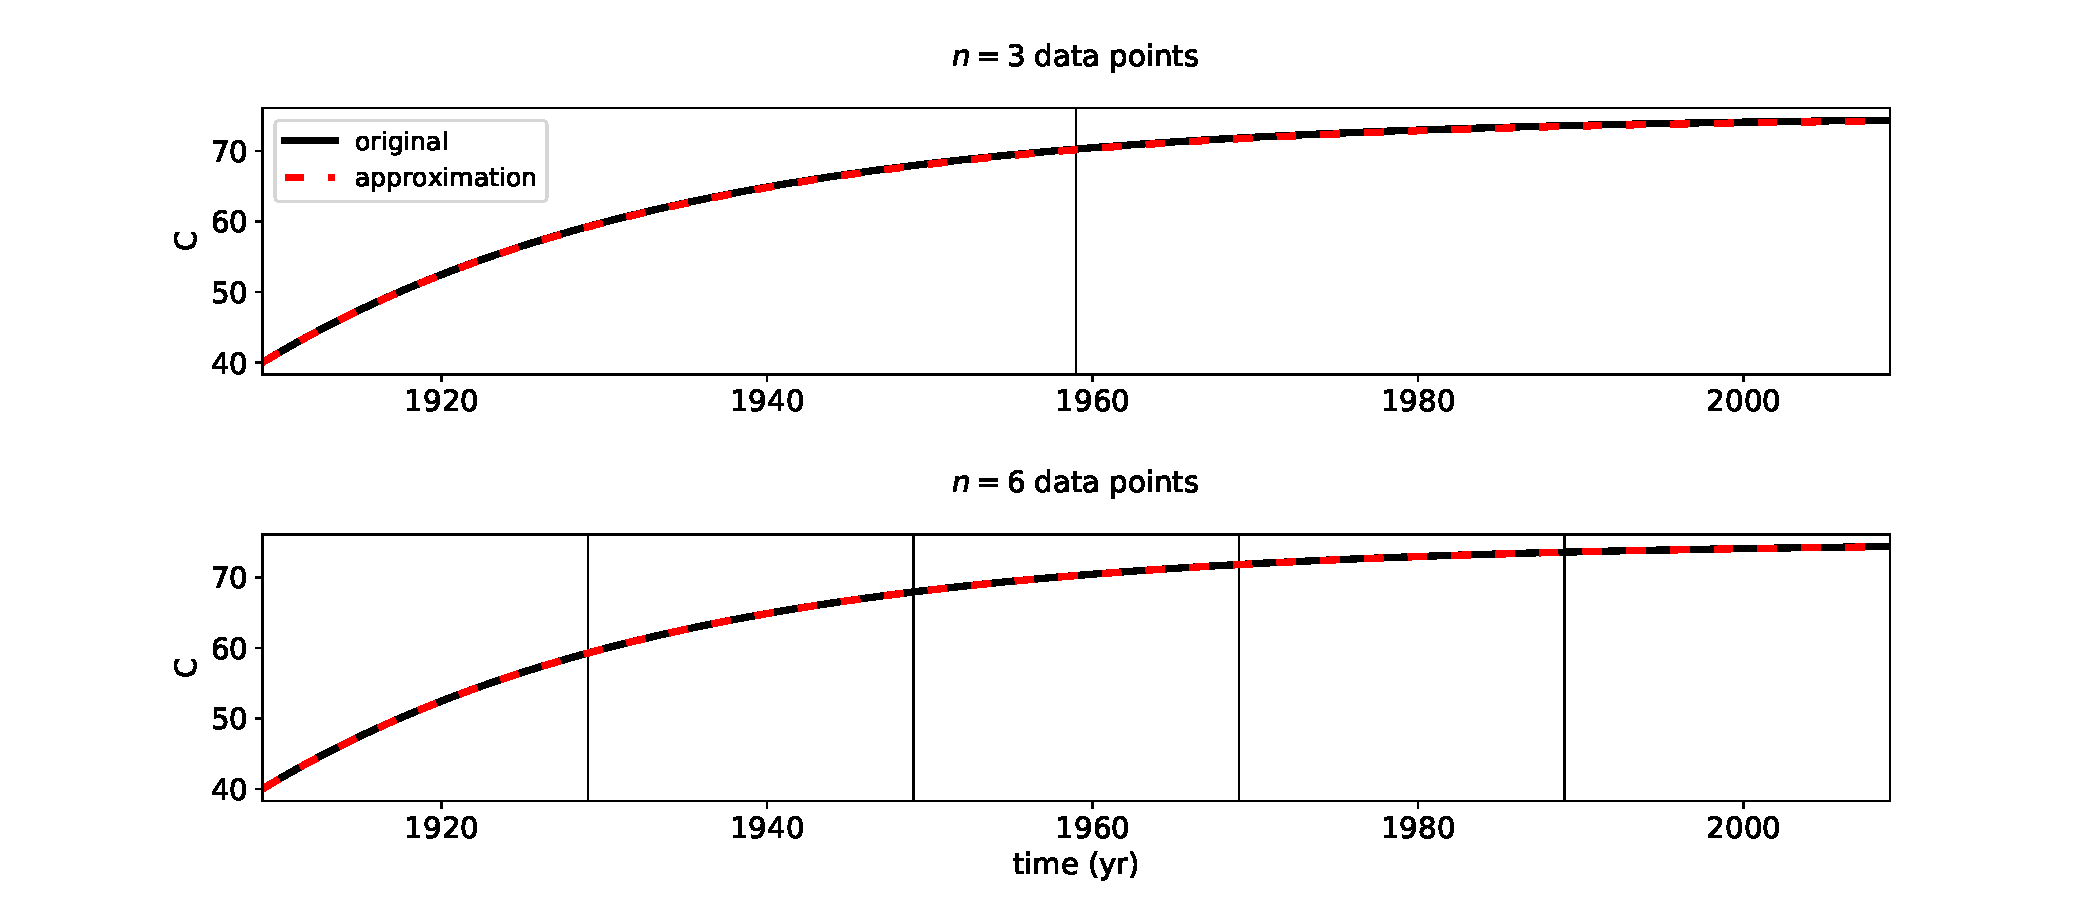
\includegraphics[width=1.0\linewidth]{figs/interpol_pwc_1_auton.pdf}
    \caption{C stocks over time for a one-pool system with constant inputs and cycling rates.
        The solid black lines represents the carbon content of the original system \eqref{eqn:CS_one_dim_example_auton}, the dashed red lines represents the carbon content obtained with the CTA.
        Different panels represent a different number of given equidistant data points, represented by vertical lines.
        }
    \label{fig:CS_one_dim_example_auton}
\end{figure}        

However, the CTA can give approximations with large errors in the time-dependent case. 
Consider the one compartment system with time-dependent inputs beginning in year 1909

\begin{equation}\label{eqn:CS_one_dim_example}
    \begin{aligned}
        \deriv{t}\,C(t) &= -0.04\,C(t) + \left[3+\sin(t/20)\right],\quad t>1919,\\
        C(1919) &= 40.
    \end{aligned}
\end{equation}
 The CTA improves with increasing number $n$ of data points used in the approximation (Figure \ref{fig:CS_one_dim_example}).
 For small number of data points, the CTA can miss important dynamics occurring inside the time step. For instance, for the reconstruction using time steps of 30 years, the convexity of the curve is completely different between the original model and the reconstruction. Therefore, care must be taken in using the CTA when important changes in dynamics occur inside the time step. 

\begin{figure}[htbp]
    \centering 
    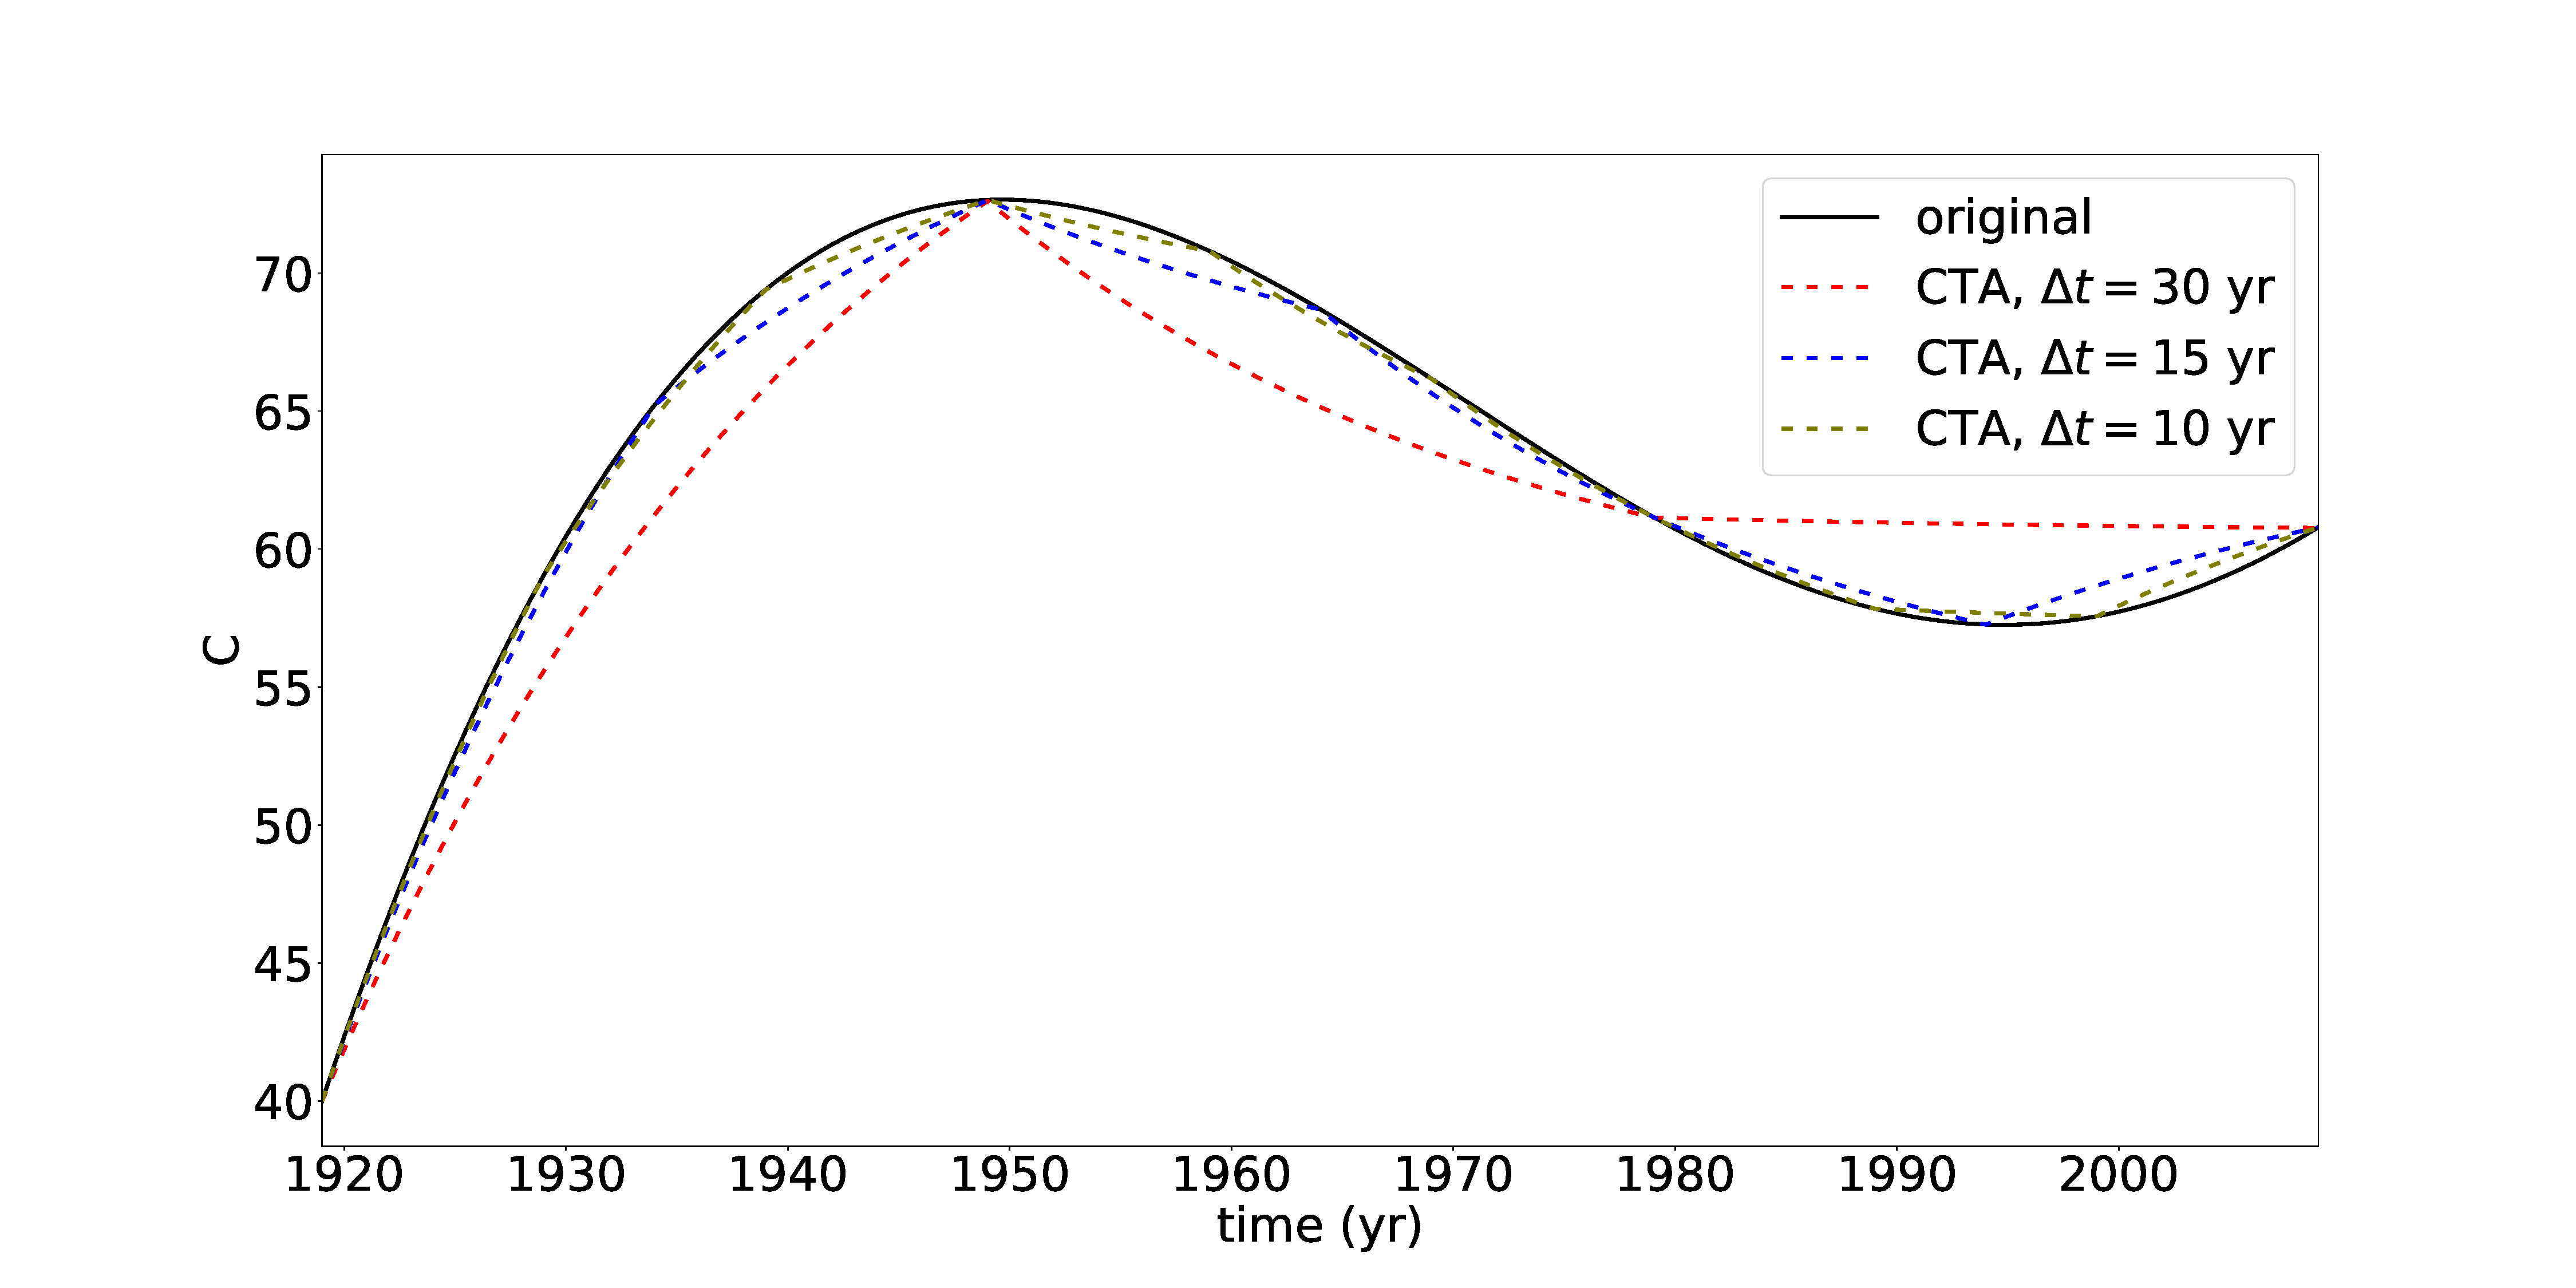
\includegraphics[width=1.0\linewidth]{figs/interpol_pwc_1.pdf}
    \caption{Transient C stocks of the one-compartment system with time-dependent inputs reconstructed by CTA for different data time steps $\Delta t$.
    Mean annual absolute bias is $\SI{3.92}{\percent}$, $\SI{0.96}{\percent}$, and $\SI{0.43}{\percent}$ for $\Delta{t} = \SI{30}{\yr}$, $\SI{20}{\yr}$, and $\SI{10}{\yr}$, respectively.
    The solid black line represents the carbon content of the original system \eqref{eqn:CS_one_dim_example}, the dashed lines represent the carbon contents of the CTAs with different time steps.}    
    \label{fig:CS_one_dim_example}
\end{figure}        


\subsection{Multi-compartment test}
    As a preliminary test before demonstrating the approach for the full ELMv1-ECA model reconstruction, we evaluated the approach for several configurations of multiple C pools and nonlinear time dependencies. We found that the accuracy of the CTA approach does not depend on the number of pools or the nonlinear time dependencies. The time step required for accurate reconstruction depends on the frequency of the forcing and non-linear interactions among pools. For example, consider a two compartment system, which can represent the dynamics of a fast and a slow soil carbon pool \cite{Andren1997}, initialized at year $t=1909$, and propagated for 110 years:
    
    \begin{equation}\label{eqn:CS_two_dim_example}
        \begingroup\makeatletter\def\f@size{10}\check@mathfonts
        \begin{aligned}
            \deriv{t}\,\begin{pmatrix} C_1(t) \\ C_2(t) \end{pmatrix} &= 
            \begin{pmatrix} -\gamma_1(t) & 0.5\,\gamma_2 \\ \gamma_1(t) & -\gamma_2 \end{pmatrix} \,
            \begin{pmatrix} C_1 \\ C_2 \end{pmatrix} +  
            \begin{pmatrix} 0.5 \\ 0.5 + 0.5\,\sin(t/100) \end{pmatrix},\\
            \begin{pmatrix} C_1(1909) \\ C_2(1909) \end{pmatrix} &=
            \begin{pmatrix} 40 \\ 0 \end{pmatrix},
        \end{aligned}
        \endgroup
    \end{equation}
    where $\gamma_1(t)=0.1+0.05\,\sin(0.1\,t)$, $\gamma_2=0.05$.
    
     In this case, data from the original model extracted at 5 yr time steps leads to a very accurate CTA, whereas coarser temporal time steps lead to progressively worse approximations (Figure \ref{fig:CS_two_dim_example}).
    \begin{figure}[htbp]
        \centering 
        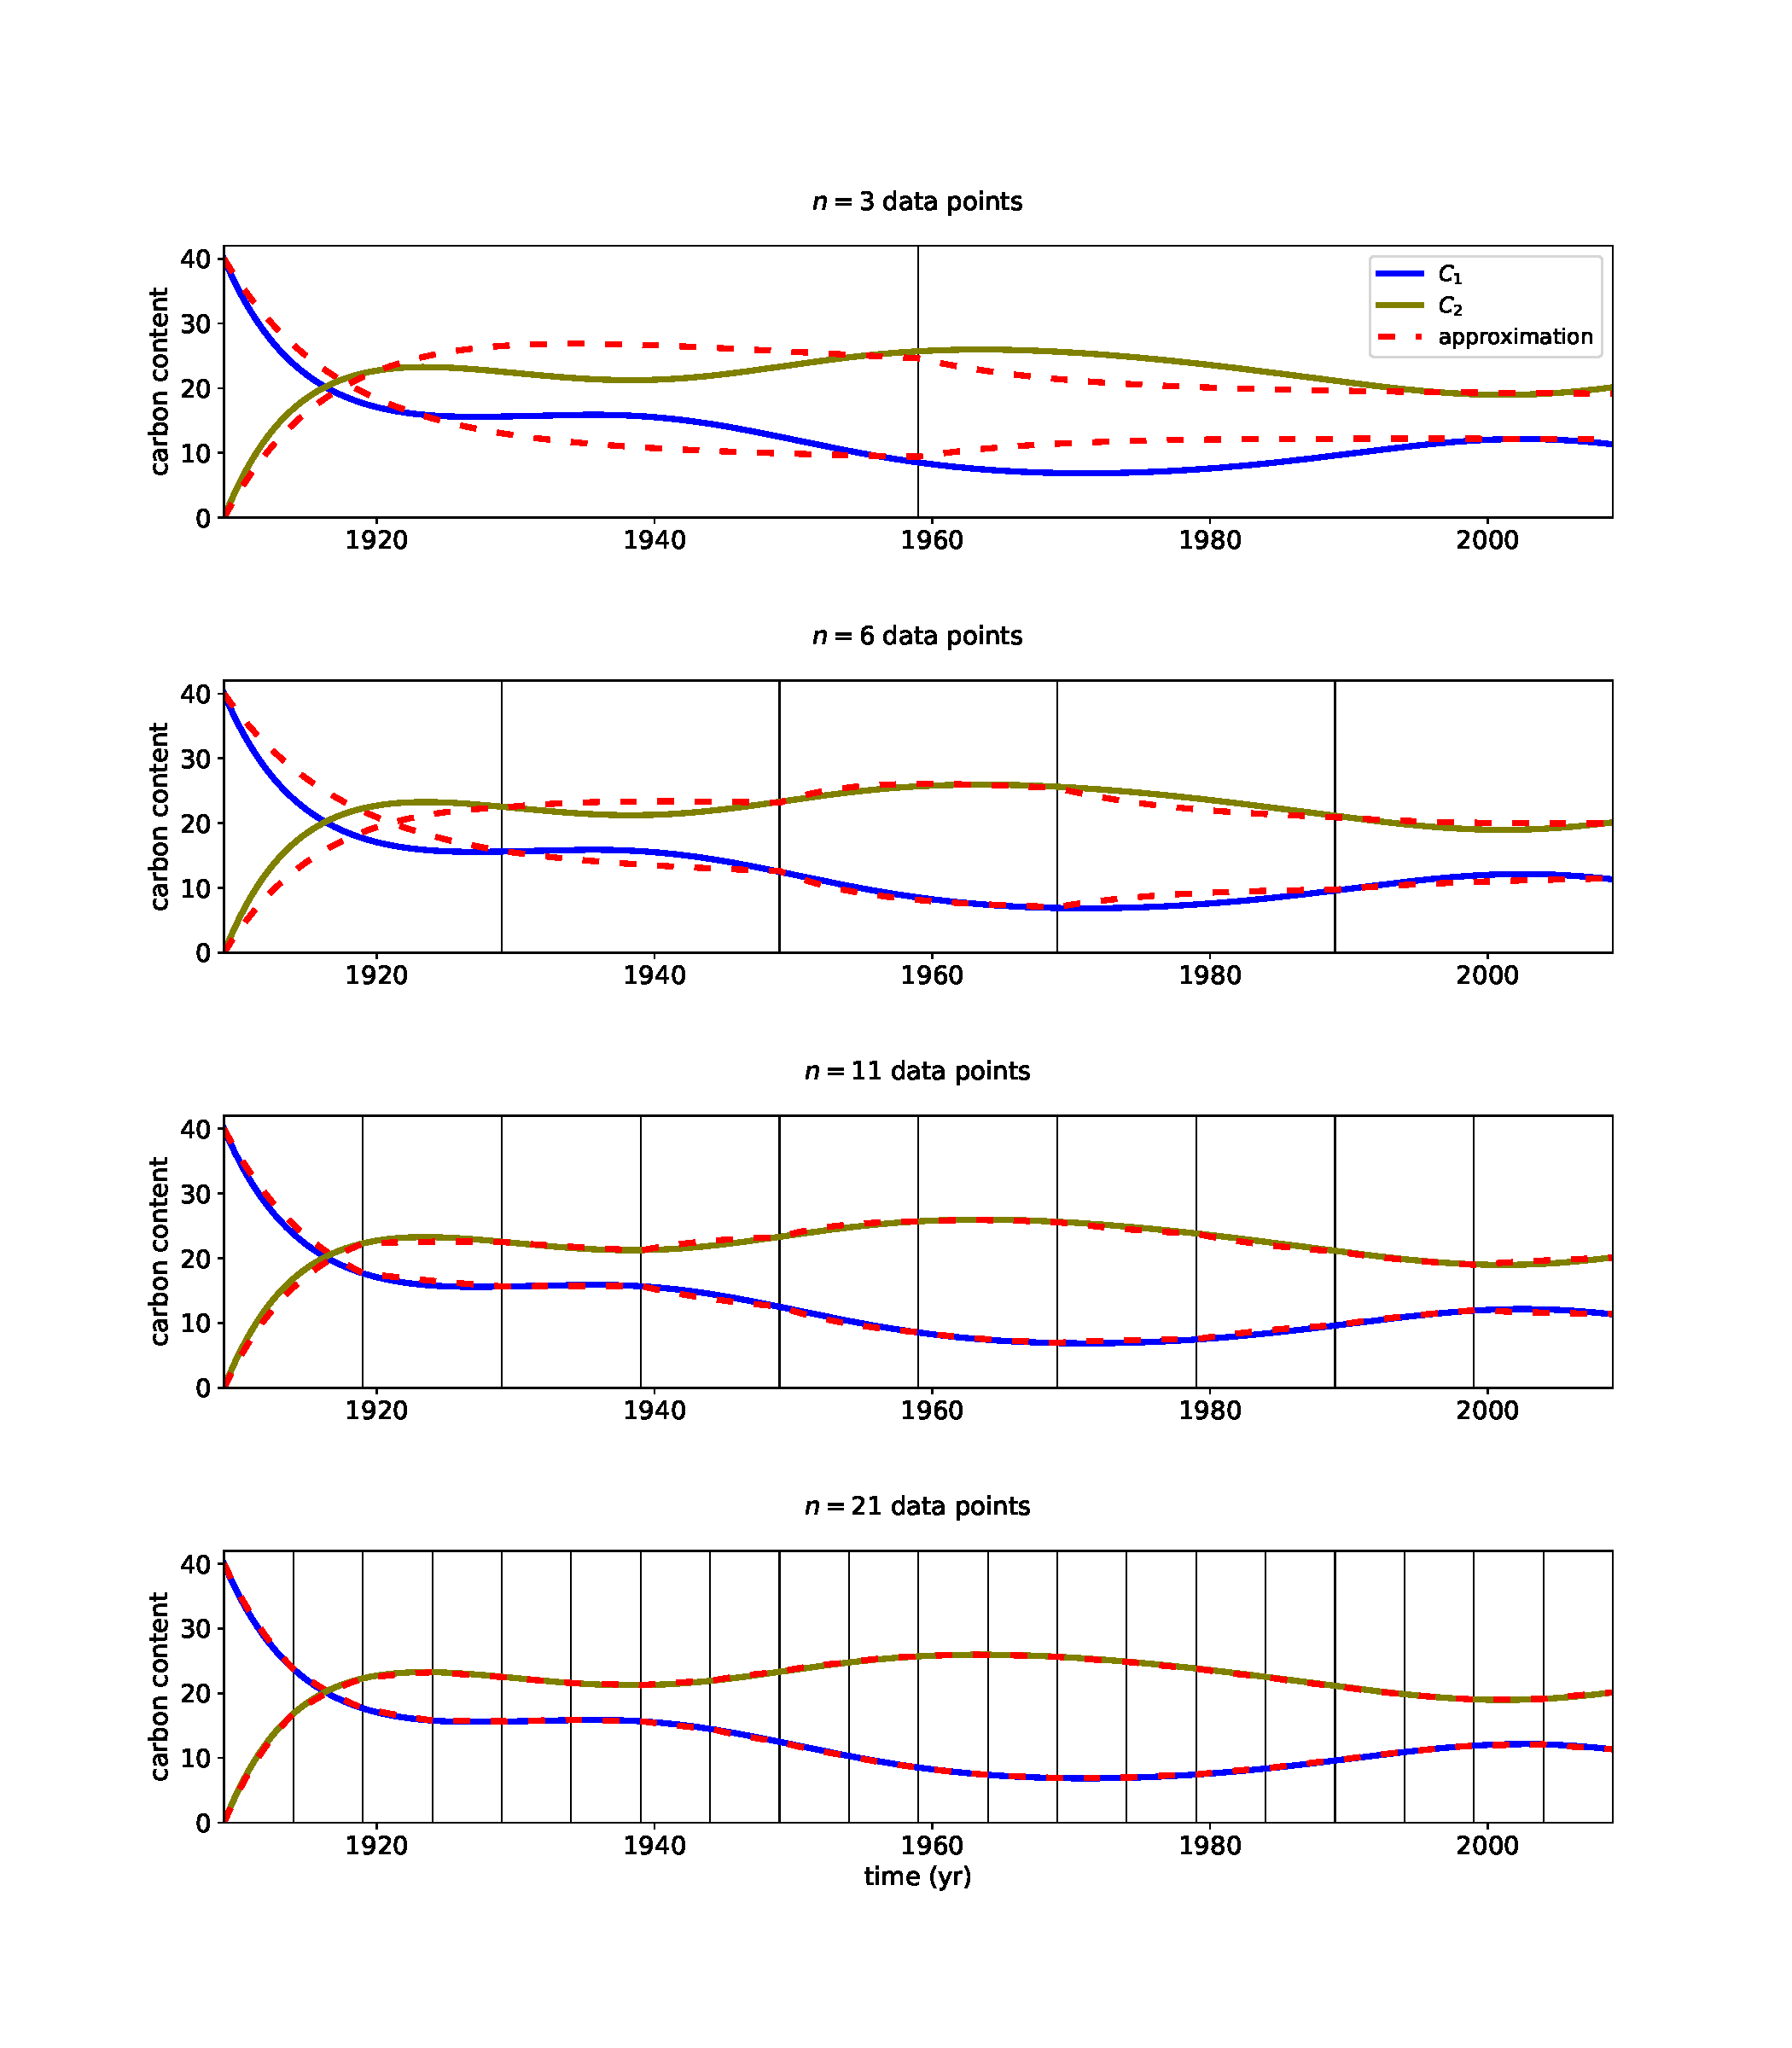
\includegraphics[width=1.0\linewidth]{figs/interpol_pwc_2.pdf}
        \caption{C stocks over time.
            The solid blue and olive curves represent the carbon contents of the two compartments of the original system \eqref{eqn:CS_two_dim_example}, the dashed red lines represent the respective CTAs. Different panels represent different numbers of given equidistant data points, represented by vertical lines.
            }
        \label{fig:CS_two_dim_example}
    \end{figure}        

\subsection{ELMv1-ECA approximation}
As long as the time-step is short enough, we can use either CTA or DTA to reconstruct the ELMv1-ECA model. CTA is generally more demanding in terms of computations because it needs to solve a system of ODEs for each time step. For practical reasons, we present here results using the DTA approach as described previously, compute radiocarbon values for all pools, and compare with the computations of radiocarbon performed in the original model. To evaluate errors related to the size of the time step, we performed simulations using 1- and 10-day ELMv1-ECA model outputs of $^{12}$C inputs, fluxes between soil pools, and atmospheric $\Delta^{14}$C. 

Our DTA accurately reproduced the ELMv1-ECA bulk soil  $^{12}$C and $\Delta^{14}$C values across the three sites and at all soil depths (Figure \ref{fig:depthProfiles}). The bulk soil $\Delta^{14}$C values shown in Figure \ref{fig:depthProfiles} combined seven SOM component pools (coarse woody debris (CWD); metabolic, cellulose, and lignin litter pools (Litter 1, 2, and 3, respectively); fast, intermediate, and passive soil pools (Soil 1, 2, and 3, respectively)), which were separately reproduced with the DTA. The mean absolute biases were $0.0003$\%, $0.0014$\% and $0.0003$\% for soil, litter, and coarse woody debris, respectively.

\begin{figure}[htbp]
        \centering 
        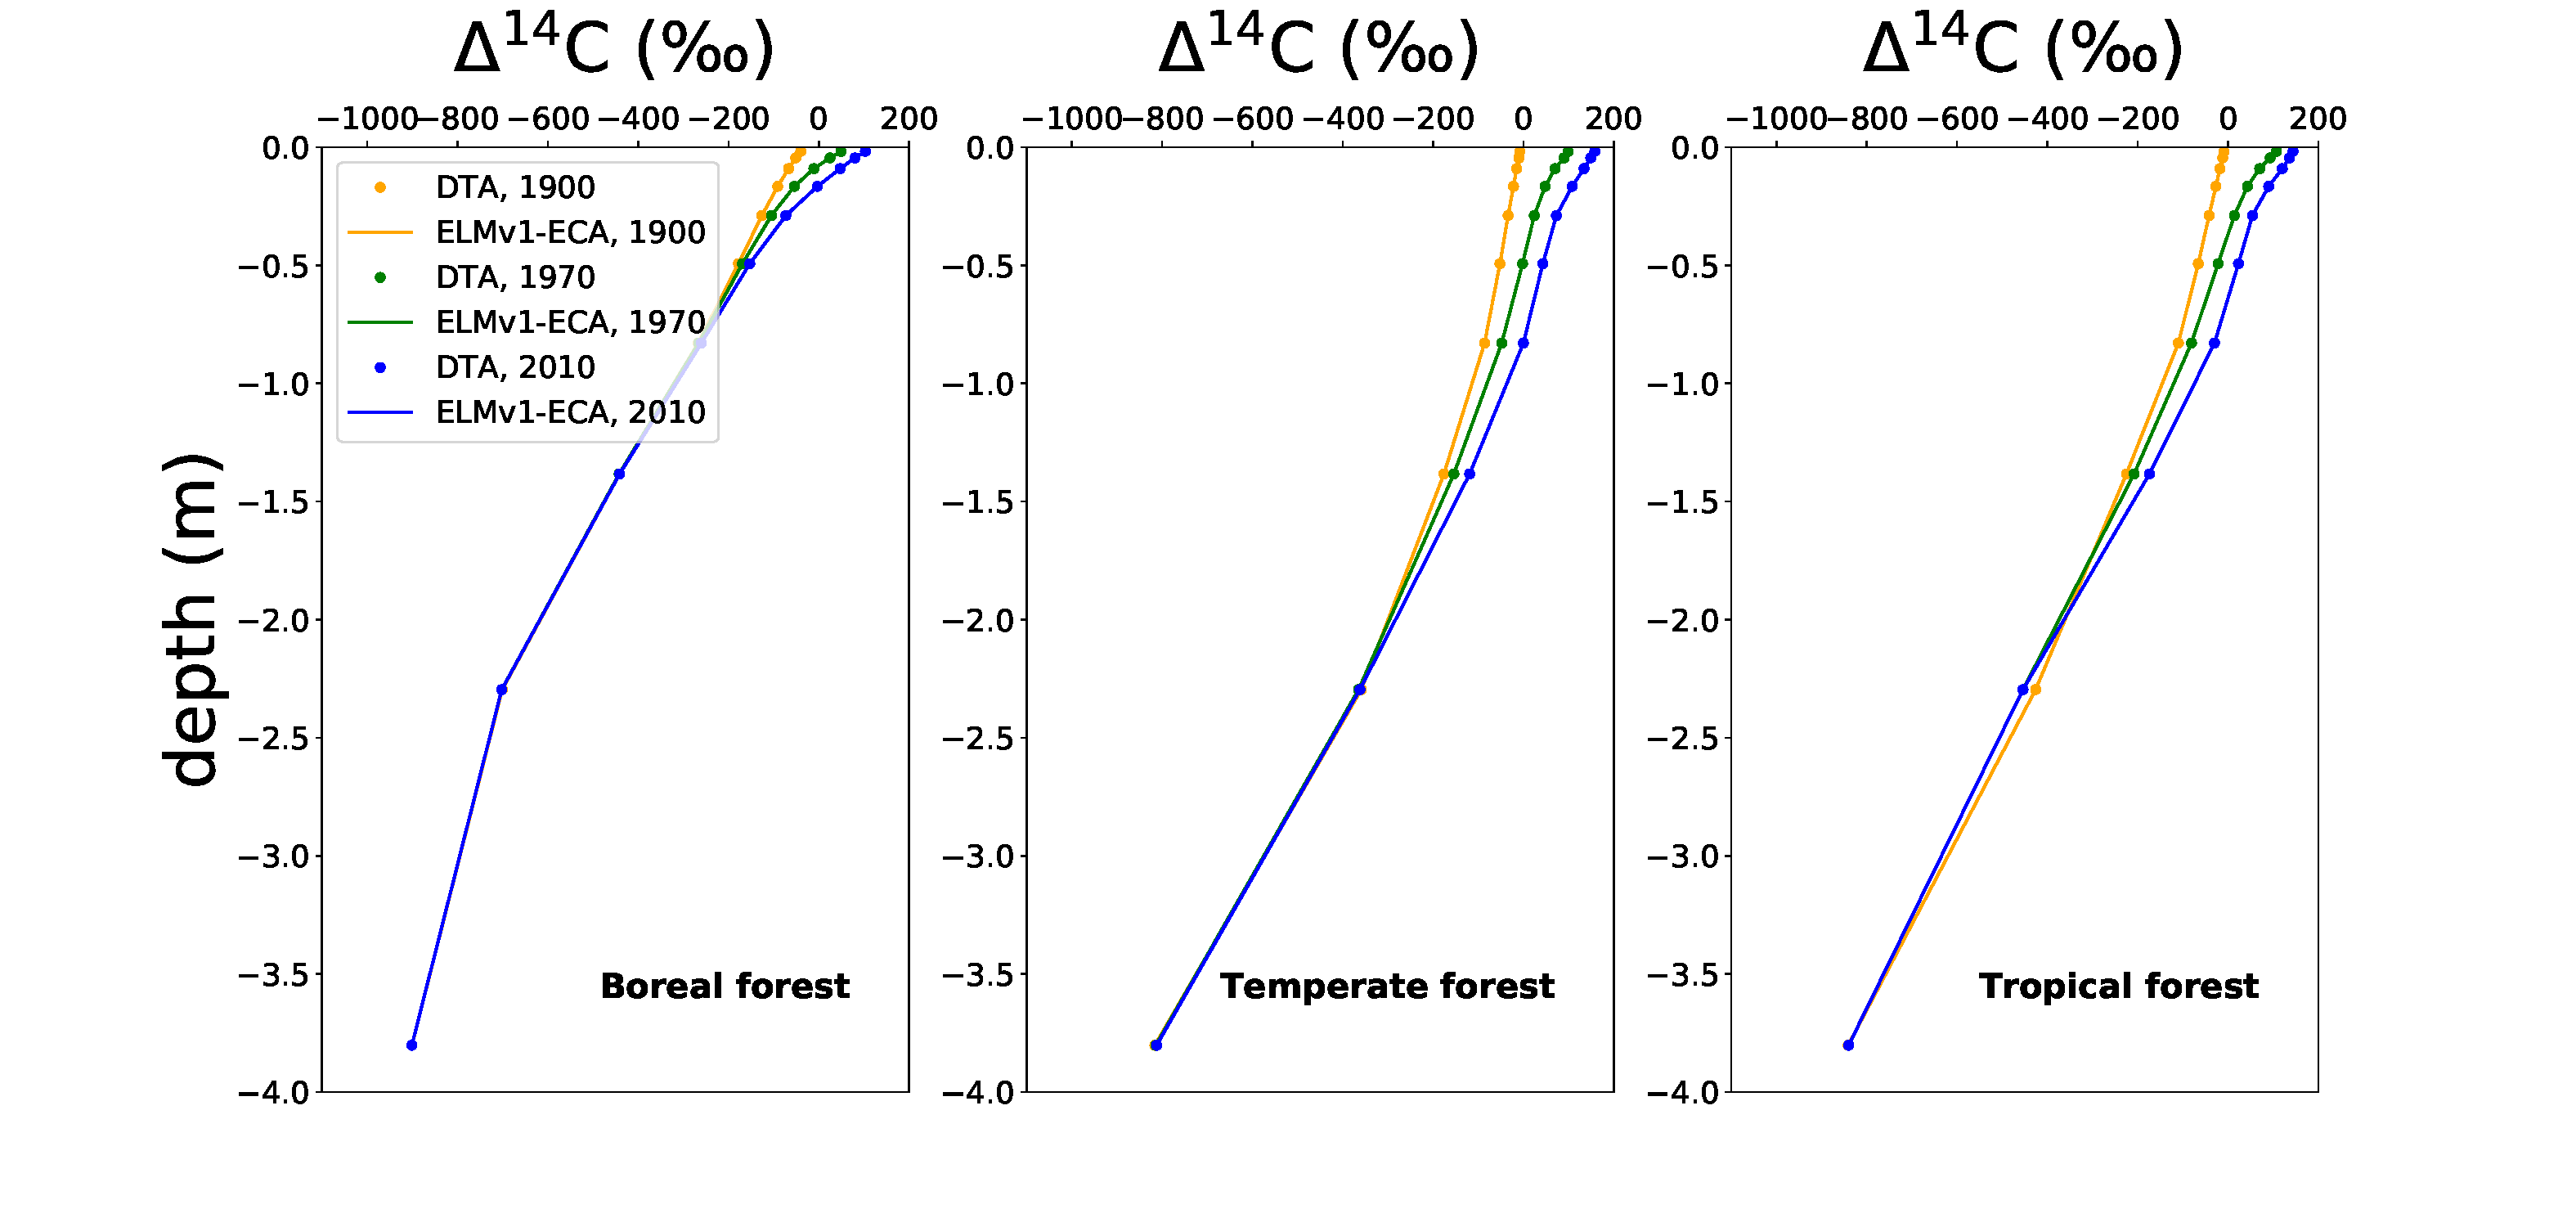
\includegraphics[width=1.1\linewidth]{figs/depth_profile_10.pdf}
        \caption{DTA using 10-day time step and ELMv1-ECA modeled $\Delta^{14}$C values with depth in 1900, 1970, and 2010. The mean absolute DTA bias is less than $0.001$\% for $\Delta^{14}$C in soils across all sites. Sites (left to right): Boreal, Temperate, Tropical. $\Delta^{14}$C values decrease with depth, and become more enriched post-1960s as they take up bomb-derived $^{14}$C from the atmosphere.
        \label{fig:depthProfiles}
        }
\end{figure}      
             

The DTA also accurately reproduced temporal variability of ELMv1-ECA modeled $\Delta^{14}$C values for all these pools over the 110 year simulation from 1901 to 2010 (Fig. \ref{fig:poolsOverTime}). For all sites, the mean absolute error was $<0.001$\% for soil carbon stocks and $\Delta^{14}$C values at all depths (Table \ref{tab:ErrorRatios}). These extremely low reconstruction errors are well within model uncertainty and far less than within-gridcell observed spatial heterogeneity of soil carbon stocks and radiocarbon values \cite{Chen2009JGR, Lawrence2019}, therefore, tolerable within the context of soil C modeling.

During the 1960s, the radiocarbon concentration in the atmosphere increased sharply due to nuclear weapons testing (generally known as the bomb spike). The CWD, litter, and fast soil pools responded relatively rapidly to this change, as atmospheric $^{14}$CO$_2$ rapidly cycled through these pools. This bomb carbon $^{14}$C signal was also evident in the top meter of soil (Figure \ref{fig:depthProfiles}). In contrast, the deeper and slower soil pools (i.e., intermediate and passive) had a more lagged and damped response to the atmospheric bomb-radiocarbon perturbation.

\begin{figure}[htbp]
        \centering 
        \vspace{-8em}
        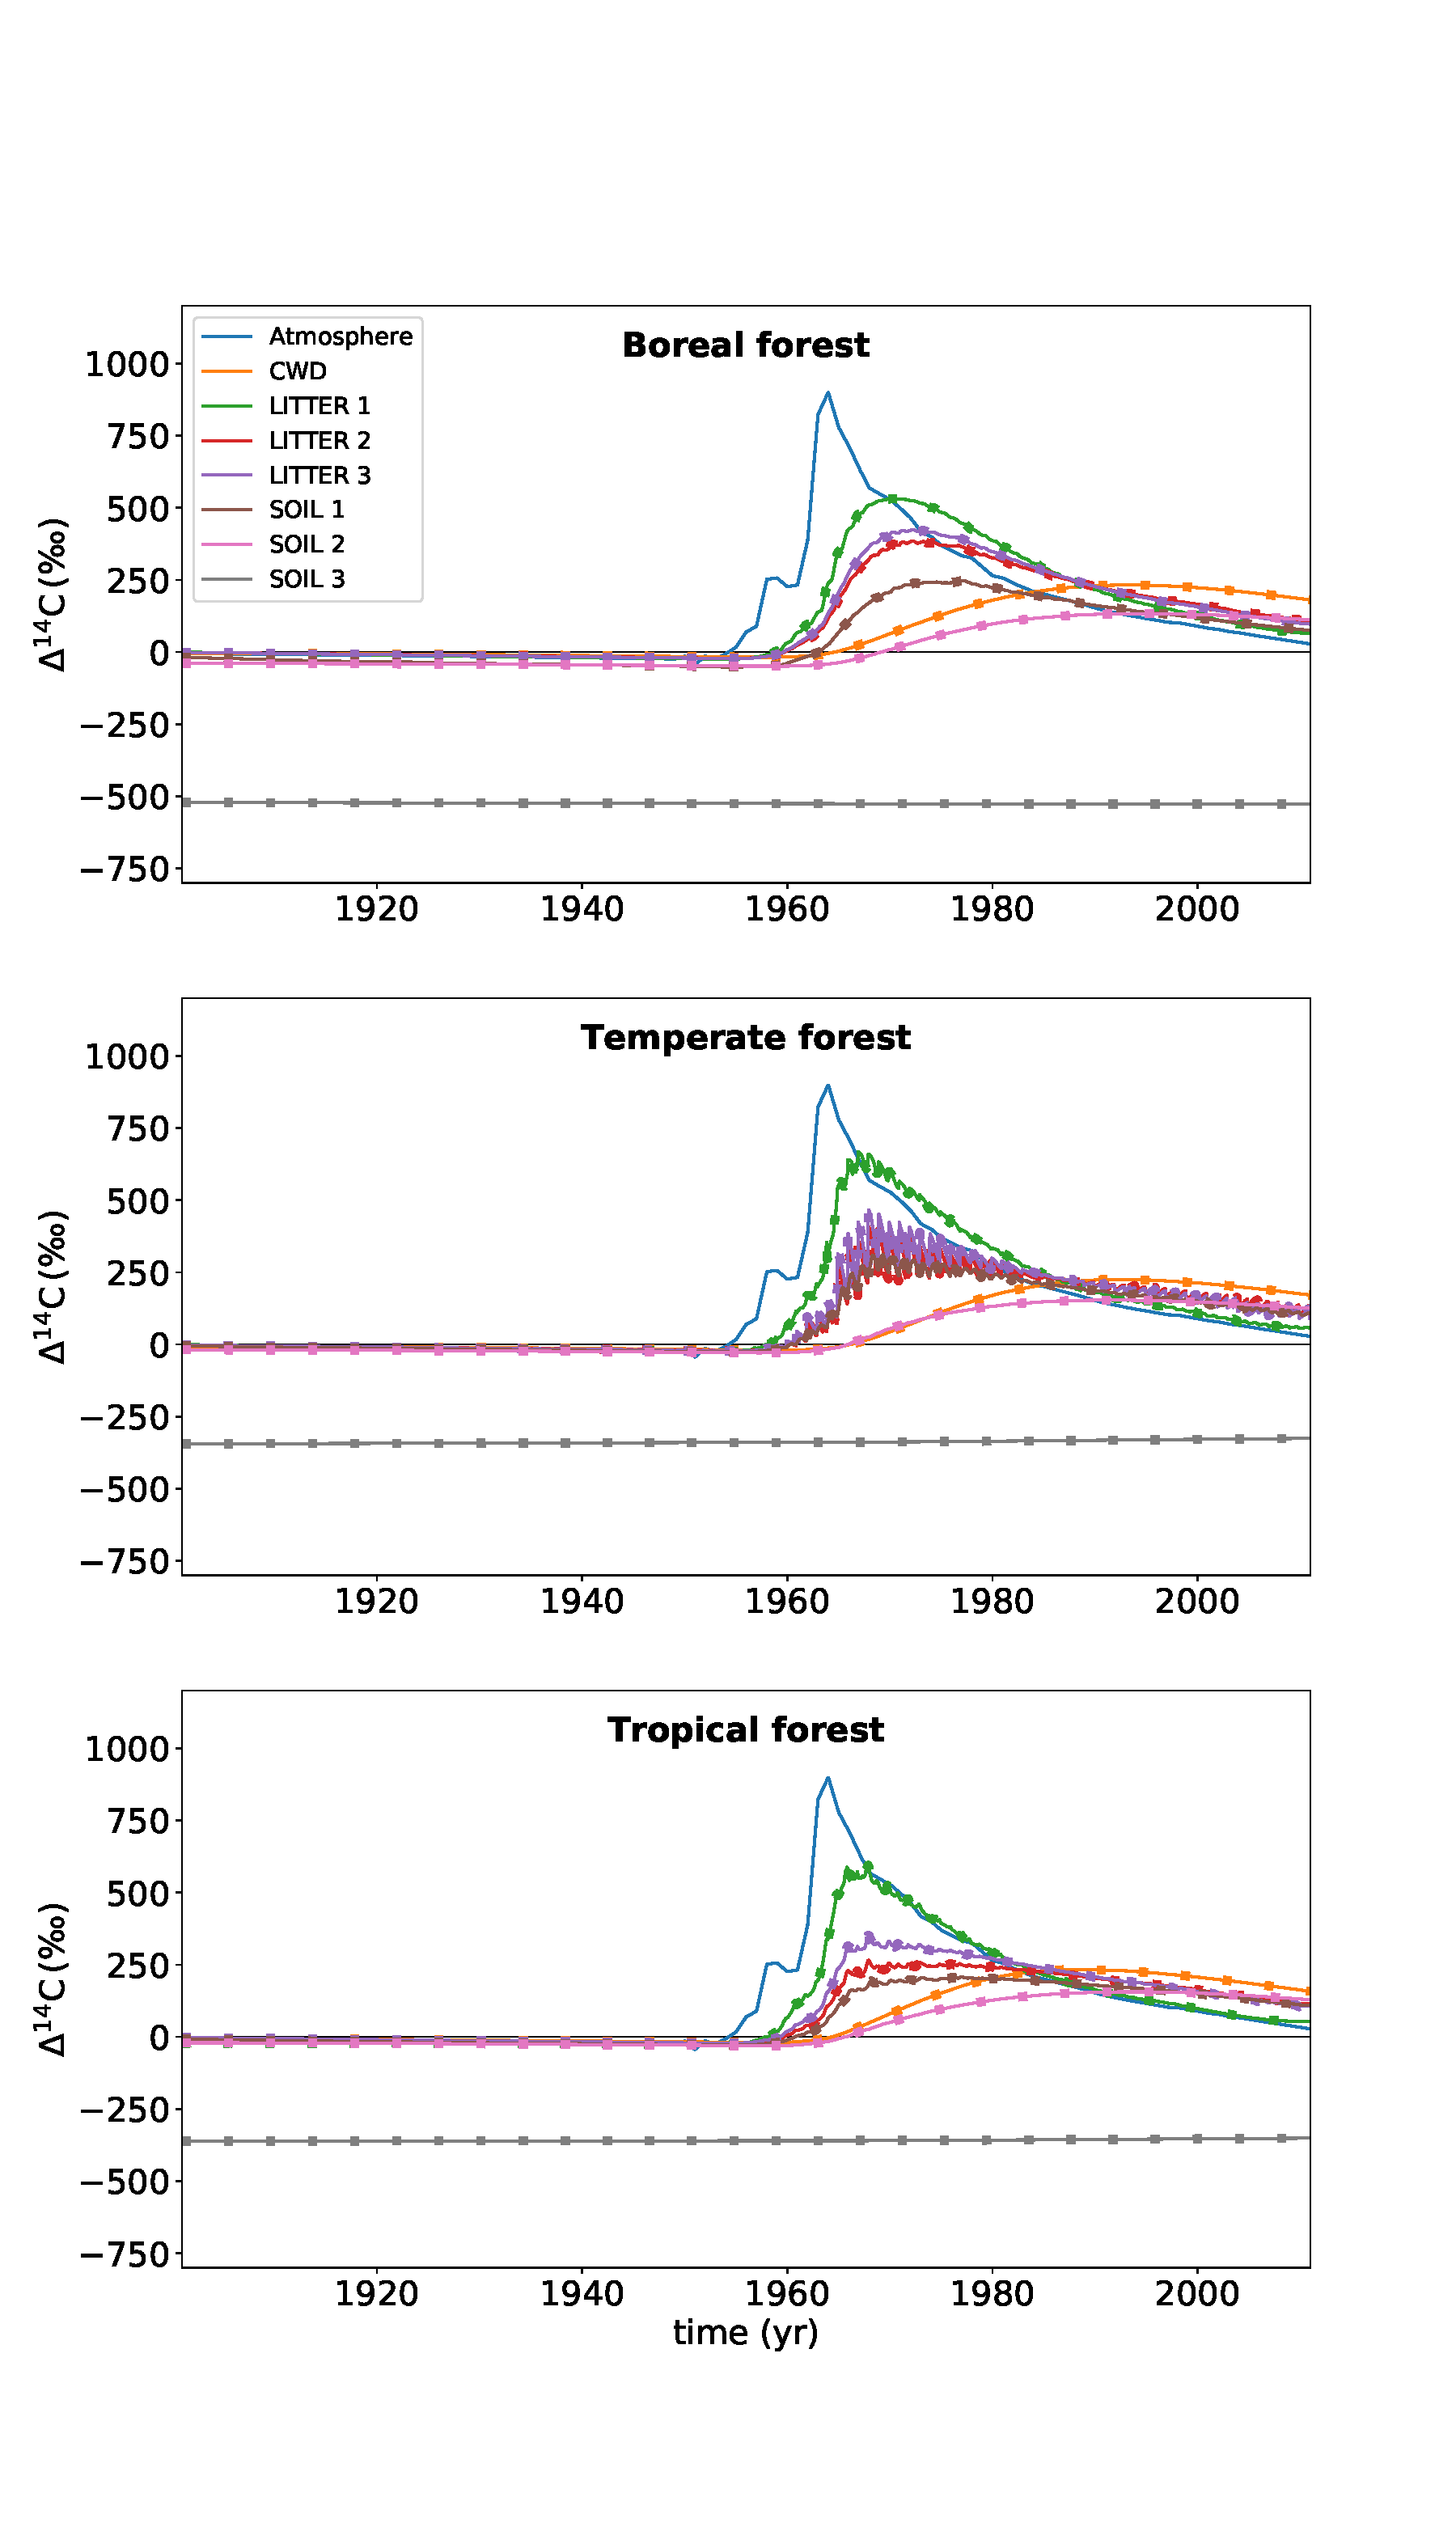
\includegraphics[width=0.9\linewidth]{figs/Delta_14C_through_time_per_pools_10.pdf}
        \vspace{-4em}
        \caption{$\Delta^{14}$C values in the different pools aggregated for all depths through time (Lines: ELMv1-ECA; dots: DTA using 10-day time step). Sites (top to bottom): Boreal, Temperate, and Tropical forests. LITTER 1,2,3 denote metabolic, cellulose, and lignin litters. SOIL 1,2,3 are fast, median, and passive soil pools. Atmospheric $\Delta^{14}$C values (blue) increase in response to nuclear bomb testing in the 1960s. Fast cycling pools respond more rapidly to the atmospheric $\Delta^{14}$C changes. Slower cycling pools show a lagged and damped response. Differences in DTA and ELMv1-ECA modeled values are imperceptible in this figure.
        \label{fig:poolsOverTime}
        }
    \end{figure}    
    
    % Is this figure showing both the computed values and the ELM values on top of each other? Or only the computed values. It is unclear from the legend ...although we know they would look the same, this should be clarified in the legend
    

Although the relative errors were extremely low across all pools over time, the percent error was larger for the CWD and litter pools than for the soil pools, with the error in the litter pool reaching a maximum during the  bomb-spike period at around 0.2\% (Fig \ref{fig:10dayErrorOverTime}). The mean absolute percent errors for DTA $^{14}$C values were, in most cases, at least two orders of magnitude larger than those for $^{12}$C across sites and pools (Table \ref{tab:ErrorRatios}). The DTA $^{14}$C error increased for larger time steps, being an order of magnitude larger for CWD and litter pools in the 10-day versus 1-day time step cases. However, the mean absolute percent error for the 10-day time step case remained very low: $< 1 \times 10^{-4}\,\%$ for $^{12}$C and $<0.01\,\%$ for $^{14}$C for all pools across different sites (Table \ref{tab:ErrorRatios}), remaining well within model uncertainty bounds and soil heterogeneity.

\begin{figure}[htbp]
        \centering 
        %\vspace{-8em}
        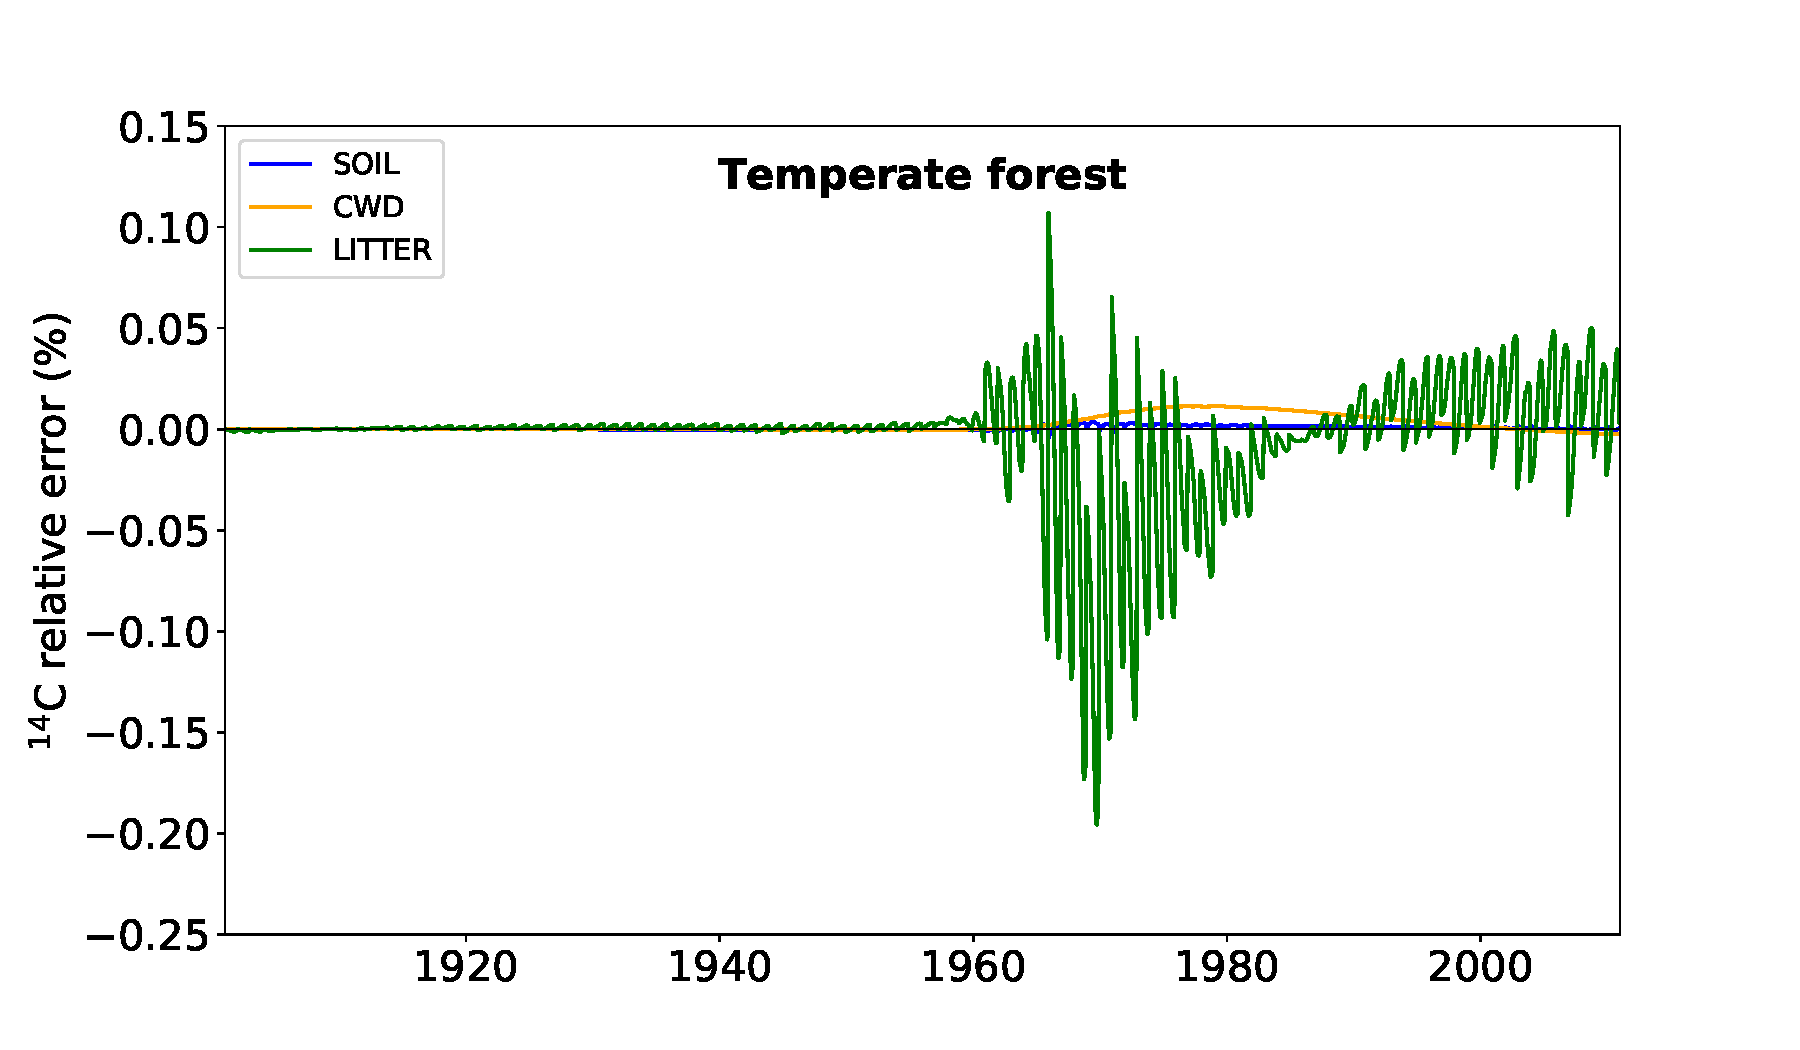
\includegraphics[width=1.0\linewidth]{figs/C14_through_time_rel_err_10.pdf}
        %\vspace{-4em}
        \caption{Relative error in radiocarbon values for CWD, aggregated litter, and soil pools over time for the temperate forest site. $^{14}$C relative error is approximately two orders of magnitude larger than $^{12}$C error, but is always small in comparison to model uncertainty and spatial heterogeneity \cite{Chen2009JGR, Lawrence2019}. The largest biases in the litter pool follow the bomb spike in atmospheric $^{14}$C concentrations and vary seasonally.}
        \label{fig:10dayErrorOverTime}
\end{figure}    

\begin{sidewaystable}
%\begin{table}[htbp]
\caption{Relative error and error ratios of a 10-day and a 1-day timestep reconstruction of ELMv1-ECA.}
\begin{tabular}{lrrrp{0.2cm}lrrrp{0.2cm}lrrr}
\multicolumn{4}{l}{\textbf{Relative error for 10 day timestep (\%):}}  &  & \multicolumn{4}{l}{\textbf{Relative error for 1 Day timestep (\%):}} &  & \multicolumn{4}{l}{\textbf{Ratio of 10-day to 1-day errors}} \\ 
${}^{12}$\textbf{C} &  & &  &  & ${}^{12}$\textbf{C} &  & & &  & ${}^{12}$\textbf{C} &  &  &  \\ 
 & \multicolumn{1}{c}{CWD} & \multicolumn{1}{c}{Litter} & \multicolumn{1}{c}{Soil} &  &  & \multicolumn{1}{c}{CWD} & \multicolumn{1}{c}{Litter} & \multicolumn{1}{c}{Soil} &  &  & \multicolumn{1}{c}{CWD} & \multicolumn{1}{c}{Litter} & \multicolumn{1}{c}{Soil} \\ 
Boreal & \num{1.21e-04} & \num{2.48e-03} & \num{2.28e-06} &  & 
Boreal & \num{1.21e-04} & \num{2.48e-03} & \num{2.28e-06} &  & 
Boreal & \num{1.0} & \num{1.0} & \num{1.0} \\ 
Temperate & \num{9.61e-07} & \num{1.22e-05} & \num{1.34e-06} &  & Temperate & \num{9.61e-07} & \num{1.22e-05} & \num{1.34e-06} &  & Temperate & \num{1.0} & \num{1.0} & \num{1.0} \\ 
Tropical & \num{1.04e-06} & \num{3.78e-06} & \num{1.03e-06} &  & Tropical & \num{1.03e-06} & \num{3.76e-06} & \num{1.06e-06} &  & Tropical & \num{1.0} & \num{1.0} & \num{1.0} \\ 
\\ 
${}^{14}$\textbf{C} &  & & &  & ${}^{14}$\textbf{C} &  & & &  & ${}^{14}$\textbf{C}  \\ 
Boreal & \num{2.39e-03} & \num{6.40e-03} & \num{2.63e-04} &  & 
Boreal & \num{2.62e-04} & \num{2.34e-03} & \num{3.68e-04} &  & 
Boreal & \num{9.1} & \num{2.7} & \num{0.7} \\ 
Temperate & \num{2.48e-03} & \num{1.41e-02} & \num{6.46e-04} &  & Temperate & \num{2.55e-04} & \num{1.41e-03} & \num{2.56e-04} &  & Temperate & \num{9.7} & \num{10.0} & \num{2.5} \\ 
Tropical & \num{2.79e-03} & \num{4.30e-03} & \num{6.17e-04} &  & Tropical & \num{2.96e-04} & \num{4.77e-04} & \num{2.73e-04} &  & Tropical & \num{9.4} & \num{9.0} & \num{2.3} \\ 
\\ 
\multicolumn{4}{l}{\textbf{Ratio of ${}^{14}$C error to ${}^{12}$C error}} &  & \multicolumn{4}{l}{\textbf{Ratio of ${}^{14}$C error to ${}^{12}$C error}} \\
Boreal & \num{20} & \num{3} & \num{115} &  & 
Boreal & \num{2} & \num{1} & \num{161} \\
Temperate & \num{2578} & \num{1155} & \num{482} &  & 
Temperate & \num{262} & \num{116} & \num{195}\\
Tropical & \num{2686} & \num{1138} & \num{599} &  & 
Tropical & \num{288} & \num{127} & \num{258}\\
\end{tabular}
\label{tab:ErrorRatios}
%\end{table}
\end{sidewaystable}

\subsection{Performance and future application}
Using a 1-day time step, the DTA accurately matched ELMv1-ECA modeled $\Delta^{14}$C values ($<$0.001\% relative error for most sites and C pools). Although the error rate increases for larger time steps, acceptable low error ($<$0.01\% relative error) is still achieved with a 10-day time step (Table \ref{tab:ErrorRatios}). These results suggest that the error would likely remain within reasonable bounds for a 30-day time step, which is common output from most ESMs.

We demonstrated here that the CTA and DTA  approaches can be applied to numerical output from land carbon models to reconstruct a linear version of the model that very closely matches the output of the original model. The approximations can then be used to simulate isotope (e.g., \textsuperscript{13}C or \textsuperscript{14}C) dynamics consistent with the original model formulation of \textsuperscript{12}C dynamics. Furthermore, the approximations can be used for both single-depth and vertically-resolved soil radiocarbon models run at different spatial and temporal resolutions. The approach is not only restricted to soils, but can also be used to reconstruct whole ecosystem carbon and isotope dynamics.  We recommend using the DTA for reconstructing ESM-scale models, since the CTA makes implicit assumptions about what the original model does between time steps, and these assumptions may  be unjustified in some cases depending on time-step size.

This DTA approach has widespread applicability, as it can be used across a range of models independent of their underlying structure. The approach does not require the model to implement additional isotope dynamics or tracers, but simply to output \textsuperscript{12}C stocks and fluxes. For maximum accuracy, all model stocks and fluxes are required (e.g., all individual transfers between all pools represented in the model). Aggregating C stocks and fluxes results in greatly increased uncertainties. However, given the uncertainties inherent in ESM land model soil carbon dynamics, reconstruction error may be lower than uncertainty in model structure and parameterization \cite{Chen2009JGR}. Error arising from pool aggregation is of particular importance when models report carbon stocks only for aggregated pools (e.g., sum of all soil carbon pools in a particular soil layer). In such cases, the original and reconstructed model will differ in structure, leading to error in the reconstruction. This error would probably depend on the number and size of pools being aggregated, and on the temporal resolution of the output. Numerical errors and instabilities may also arise from empty or very small pools. For instance, we observed larger relative errors in the relatively small deep litter and CWD pools.

%\red{Make sure to cover: (1) what is required to make the approach work (fluxes and states that affect 12C); application to existing models; (2) application to single- and multi-layer models; (3) Discussion on why 12C does better than 14c? Relatedly, why does the soil do so much better than the litter and CWD? }

The potential of this approach to produce radiocarbon predictions across models that do not explicitly represent it will allow us valuable data-model comparisons and enable use of radiocarbon as a constraint for parameter estimation \cite{He2016}

Although radiocarbon is commonly associated with C age, it cannot be directly interpreted as such in soils, due to mixing of C inputs of different ages in the open system \cite{Trumbore2016}. Instead, radiocarbon measurements and model output are primarily of value as a tracer, and for direct model-data comparison. In addition, by using a state-transition matrix approach as we did here, there is the added possibility to calculate age and transit time distributions for the system \cite{Metzler2018PNAS}. In the future, this approach could be applied to compute radiocarbon values, ages, and transit times across a suite of models and evaluate the time carbon spends in terrestrial ecosystems. This approach would provide meaningful comparisons of C ages and transit times between model structures and transient scenarios. 

In addition, the reconstruction we propose of numerical model output as a dynamical system can be used to compute other system-level diagnostics of the terrestrial carbon cycle. For instance, \citeA{Luo2017} proposed a set of diagnostics to evaluate carbon storage capacity and potential from transient simulations, and developed a framework to assess model performance based on the ability to trace particular components of ecosystems \cite{Xia2013, Luo2015}. From the numerical model reconstructions we proposed here, it is possible to perform these analyses without the need to analytically rewrite existing models in matrix form. This means that it is still possible to obtain time-dependent versions of these matrices and vectors in numeric form, without the need to explicitly write by hand all equations of the model. This can be an advantage for complex models with multiple interactions between the carbon cycle and the water, nutrient, and energy cycles. 

\section{Conclusions}
Numerical output from carbon cycle models can be used to reconstruct a linear version of the model that exactly matches the solution trajectory of the original model. This reconstruction can be used to compute other quantities not included in the original model such as isotope dynamics and other system-level metrics. The approach consists of computing a state transition matrix that contains all information of the dynamics of the system. Since available model output is always reported in discrete time steps, we proposed here two methods to approximate the original system, approximating a continuous system between time steps, or approximating a discrete dynamical system. As long as the time-step of the numerical output is sufficiently small to capture complex dynamics, both approaches provide very good approximations to the solution trajectory of the original system. 

Radiocarbon is a valuable tracer to evaluate, understand, and improve soil carbon models. However, most land models do not currently include explicit representation of soil radiocarbon dynamics, precluding comparison with observations. Here we demonstrated how continuous and discrete time approaches can reconstruct soil radiocarbon profiles using only land model \textsuperscript{12}C stocks and fluxes and atmospheric \textsuperscript{14}C values. We applied the approach here to the ELMv1-ECA model \cite{Zhu2019, Riley2018,Tang2018EI}, which explicitly represents soil organic matter \textsuperscript{14}C dynamics with seven soil pools and ten vertical layers, and showed that our approach very accurately reproduces the full model simulations (bias $<0.01$\%). The approach can also be used for the new suite of CMIP6 simulations to evaluate whether the models are accurately representing soil C age and transit time, in addition to soil carbon stock \cite{He2016, Lawrence2019}. For applications to CMIP6 models, it is required that the models report all pools and all fluxes among pools as requested in the tier-2 output requirements of C4MIP  \cite{Jones2016}.
%\section*{Acknowledgements}
\acknowledgments
Funding was provided by the Max Planck Society and the German Research Foundation through its Emmy Noether Program (SI 1953/2--1). A.M.H. received funding from the European Research Council (ERC) under the European Union’s Horizon 2020 research and innovation programme (grant agreement No. 695101 (14Constraint)). WJR and QZ were funded by the Director, Office of Science, Office of Biological and Environmental Research of the US Department of Energy under Contract No. DE-AC02-05CH11231 as part of the Regional and Global Climate Modeling (RGCM), RUBISCO SFA, and the E3SM project.

All code required to reproduce the results presented in this manuscript has been permanently archived at \url{DOI: 10.5281/zenodo.3520048}.

%\bibliographystyle{apalike}
%\bibliographystyle{gcb}
\bibliography{refs}


\end{document}